\documentclass[11pt]{report}

%% Useful packages
\usepackage[a4paper,top=3cm,bottom=3cm,left=3.5cm,right=3cm,marginparwidth=1.75cm,headheight=22pt]{geometry}
\usepackage{amsmath}
\usepackage{cite}
\usepackage{courier}
\usepackage{minted} % For highlighted source code
\usepackage[titletoc]{appendix}
\usepackage[export]{adjustbox}
\usepackage[nottoc,notlot,notlof]{tocbibind}
\usepackage[labelfont=bf, textfont=bf]{caption}
\usepackage{graphicx}
\usepackage{hyperref}
\usepackage{float}
\usepackage{setspace}
\usepackage{subfigure}
\usepackage{setspace}
\usepackage{lipsum}
\usepackage{fancyhdr} % Fancy header
\usepackage{url}
\usepackage{tabularx}
\usepackage[utf8]{inputenc}
\usepackage{mathptmx} %Times Font
\setlength{\parindent}{0em}
\usepackage{biblatex}
\usepackage{minted}

\begin{document}
\fontdimen2\font=0.5em% inter word space

%%%%%%%%%%%%%%%%%%%%%%%%%%%%%%%%%%%%%%%%%%%%%%%%%%%%%%%%%%%%%%%%%%%%%%%%%%%%%%%%%%%%%%%
% Title Page
%%%%%%%%%%%%%%%%%%%%%%%%%%%%%%%%%%%%%%%%%%%%%%%%%%%%%%%%%%%%%%%%%%%%%%%%%%%%%%%%%%%%%%%
\begin{center}
    
\includegraphics[width=.5\textwidth]{Images/uoftlogo.png}


\vspace{1.5in}

\Huge{\textbf{Friendify \\ A friend-making Application}}\\[2.5in]

\LARGE{\textbf{CSC111 Final Project}}\\[0.5in]

\normalsize{\textbf{Eeshan Narula and Avnish Pasari}}\\[0.2in]
\end{center}


\newpage 


%%%%%%%%%%%%%%%%%%%%%%%%%%%%%%%%%%%%%%%%%%%%%%%%%%%%%%%%%%%%%%%%%%%%%%%%%%%%%%%%%%%%%%%
% Table of Content
%%%%%%%%%%%%%%%%%%%%%%%%%%%%%%%%%%%%%%%%%%%%%%%%%%%%%%%%%%%%%%%%%%%%%%%%%%%%%%%%%%%%%%%
\tableofcontents
\newpage

%%%%%%%%%%%%%%%%%%%%%%%%%%%%%%%%%%%%%%%%%%%%%%%%%%%%%%%%%%%%%%%%%%%%%%%%%%%%%%%%%%%%%%%
% Introduction 
%%%%%%%%%%%%%%%%%%%%%%%%%%%%%%%%%%%%%%%%%%%%%%%%%%%%%%%%%%%%%%%%%%%%%%%%%%%%%%%%%%%%%%%

\chapter{Introduction}

The onset of COVID-19 has made it extremely hard for people to socialize and make new friends.\\

The constant quarantine and not being able to meet people, visit restaurants, go to clubs or attend social events has led to an increased social isolation amongst people. \\

This increased social isolation amongst people, if not addressed, can negatively impact the mental health and development of the concerned individual. (\href{https://www.healthline.com/health-news/people-with-covid-19-more-likely-to-develop-depression-anxiety-and-dementia\#How-the-new-coronavirus-affects-the-mind}{\color{blue}Source 1})\\

Studies have shown that loneliness is often associated with negative thoughts (cognition). Moreover, anxiety and depression may cause social withdrawal which exacerbates the loneliness and isolation associated with social distancing.
(\href{https://www.ncbi.nlm.nih.gov/pmc/articles/PMC7306546/\#:\\~:text=Quarantine\%20and\%20social\%20distancing\%20are,and\%20mental\%2Dhealth\%20related\%20repercussions}{\color{blue}Source 2})\\ 

Most humans, by nature, are social creatures. Over the past few months - repeated lock-downs, bans on public gatherings and self-imposed quarantine have severely impacted interaction amongst the people.\\

This has led to the development of fear, stress and anxiety amongst the masses during these uncertain and difficult times. Thus it becomes increasingly vital for us to interact with people (online) and keep ourselves engaged, both to preserve our mental health and also to create a positive environment for those around us (i.e. family).(\href{https://www.kff.org/coronavirus-covid-19/issue-brief/the-implications-of-covid-19-for-mental-health-and-substance-use/}{\color{blue}Source 3})\\

Interacting and connecting with people who have shared interests and hobbies can help reduce mental stress, anxiety and isolation-trauma, thus enabling people to better cope with the COVID-19 pandemic.\\

Studies have shown that online social interaction in such a time, can help rejuvenate our low spirits, improve mental health and sharpness as well as enable us to develop life-long relations with others during this time, which may have otherwise been impossible without our current technology. 
(\href{https://oaksatdenville.org/blog/benefits-social-interactions/}{\color{blue}Source 4})\\

To address this issue of adverse mental health conditions due to decreased social interaction and to provide a solution in the form of an online platform where people can find and connect with each other - {\textbf {\large We plan to design a program which would allow people connect with each other so as to find and make friends based on their shared interests and compatibility.}}

% \newpage 

%%%%%%%%%%%%%%%%%%%%%%%%%%%%%%%%%%%%%%%%%%%%%%%%%%%%%%%%%%%%%%%%%%%%%%%%%%%%%%%%%%%%%%%
% Description 
%%%%%%%%%%%%%%%%%%%%%%%%%%%%%%%%%%%%%%%%%%%%%%%%%%%%%%%%%%%%%%%%%%%%%%%%%%%%%%%%%%%%%%%
\chapter{Datasets}


{\bf Description}

~

Initially our app would not have any users registered with it.\\ 

Thus we conducted a survey where we asked people about their movies, music, games and food preferences.\\
The survey was conducted using Google forms. \\

We also asked the participants for their emails, but scrapped the part after @ to maintain privacy. The timestamp was also removed from the data-set, for the same reason. \\

The data collected has been stored in a csv file. Provided below is a picture demonstrating how the concerned csv file looks \\

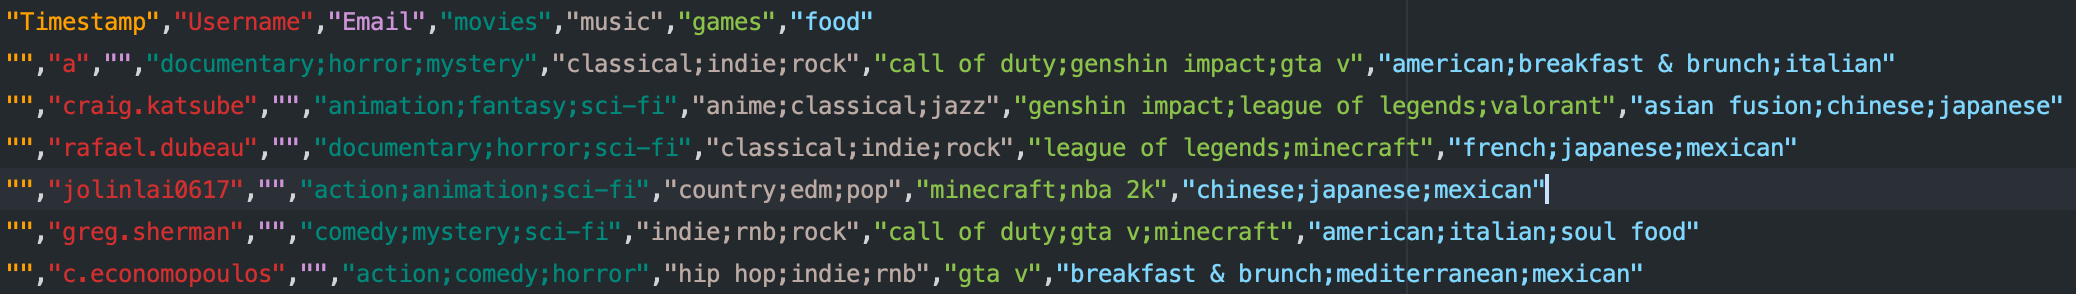
\includegraphics[scale = .4]{Images/data.png}~\\\\

{\bf Columns Used:}

\begin{itemize}
    \item Username: the column "Username" is used to identify the users.
    
    \item movies, music, games, food: Used to recommend friends to the users of the app.
\end{itemize}


\newpage 




%%%%%%%%%%%%%%%%%%%%%%%%%%%%%%%%%%%%%%%%%%%%%%%%%%%%%%%%%%%%%%%%%%%%%%%%%%%%%%%%%%%%%%%
% Computational Planning
%%%%%%%%%%%%%%%%%%%%%%%%%%%%%%%%%%%%%%%%%%%%%%%%%%%%%%%%%%%%%%%%%%%%%%%%%%%%%%%%%%%%%%%
\chapter{Computational Planning}

\section{Overview}

The App uses real world data, to recommend friends, visualize network and socialize. \\

The data contains information of all the users of the app. The information consists of the unique user ID and the preferences of the user. The preferences represent the different movies, music, food and games that the user likes. \\

This data is used to construct recommendation graphs and network graphs which consists of the users and their preferences as the vertices, with edges representing a relation between two users or a users preferences. \\

This data is stored on cloud and is accessed by our app very time a user wants to see friend recommendations, visualise their friend circle or socialize. \\

The working of the app is divided into 5 main parts:- Handling the user's data, Recommending friends, Visualizing friends circle, Searching for People, and User Interface handling. 

\newpage 

\section{Handling the Data}

All the data is stored in Google's Firebase cloud storage, as a database. The database consists of user data, identified by the unique user ID. We are using a library called firebase-admin to communicate with the cloud storage, to retrieve and set data.\\

We have created a DataHandler class (authentication.py), which configures the connection between the cloud and the app. This class is responsible to handle all the requests to the cloud. It contains the functions, to create a new user, sign in the user, load a user's data by their unique user id, set a user's data, update a user's data and many other functionalities. \\

We have tried to use the MVC architecture to handle the data in an efficient  way. The DataHandler class acts as the Model-bridge between the View controller and the Database. Both View controller and the Database interact with each other through the DataHandler.

\begin{center}
     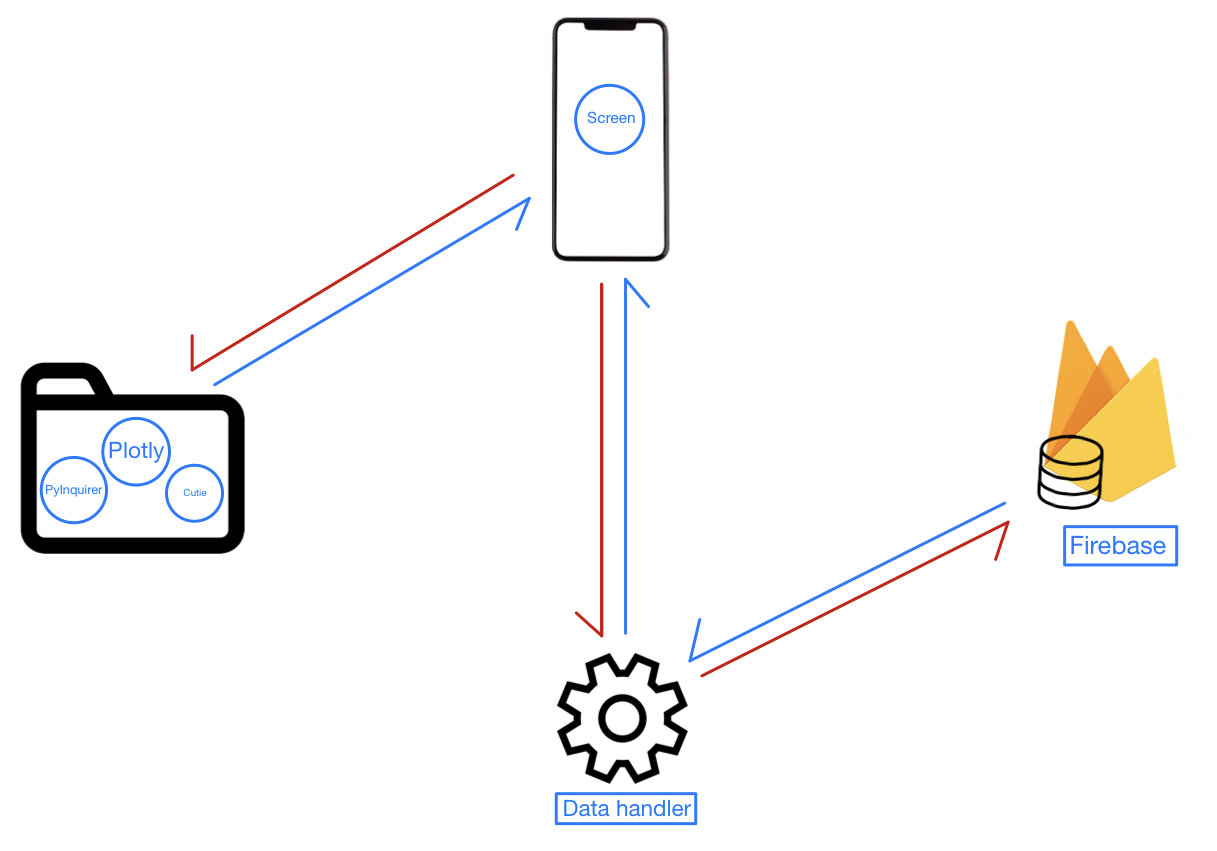
\includegraphics[scale = .28]{Images/handling.jpeg}
\end{center}

In the above figure, the screen represents the View controller. For getting data, signing in and registering, the Screen first sends a request to the DataHandler. \\

The DataHandler then send a request to the Firebase cloud server to get the data. The server responds and returns the data to the DataHandler. The DataHandler then returns this data to the Screen/View Controller. \\\\

{\bf Initial Data} ~\\

Initially there were no users, so there were no friend recommendations. Thus we conducted a survey in which approximately 50 people participated. The DataHandler class was also used to read the survey data, and register all the users to the cloud database. These 50 users were also assigned some friends according to the recommendation system.




\section{Recommending friends}

The main goal of the app is to recommend friends to the user. The app fulfills this goal by constructing recommendation and network graphs. 
~\\\\

\textbf{Constructing The Graph}

\begin{itemize}
    \item To construct the graph first we load data for all the users of the app using the DataHandler class (authentication.py). \\ 
    
    \item For each user, we create a vertex, with the unique user ID as the value of the vertex. These vertices are of type user.\\
    
    \item We would then add all the possible preferences a user can have to the graph, as a vertex. These vertices are labelled as preferences. For instance these preferences could be the type of music, type of food, movies or games the user likes.\\
    
    \item Now we would add an edge between all the users and their preferences, which would represent a user preference relation, and an edge between user and other users, which would represent friendship between the two users.  \\
    
    \item The graph is generated by the load\_friends\_graph function present in Graph class in recommendation\_graph.py \\
    
    \item This is how the graph should look like (the vertices in orange circles are the preferences, these are used to recommend friends to the user): \\
    
        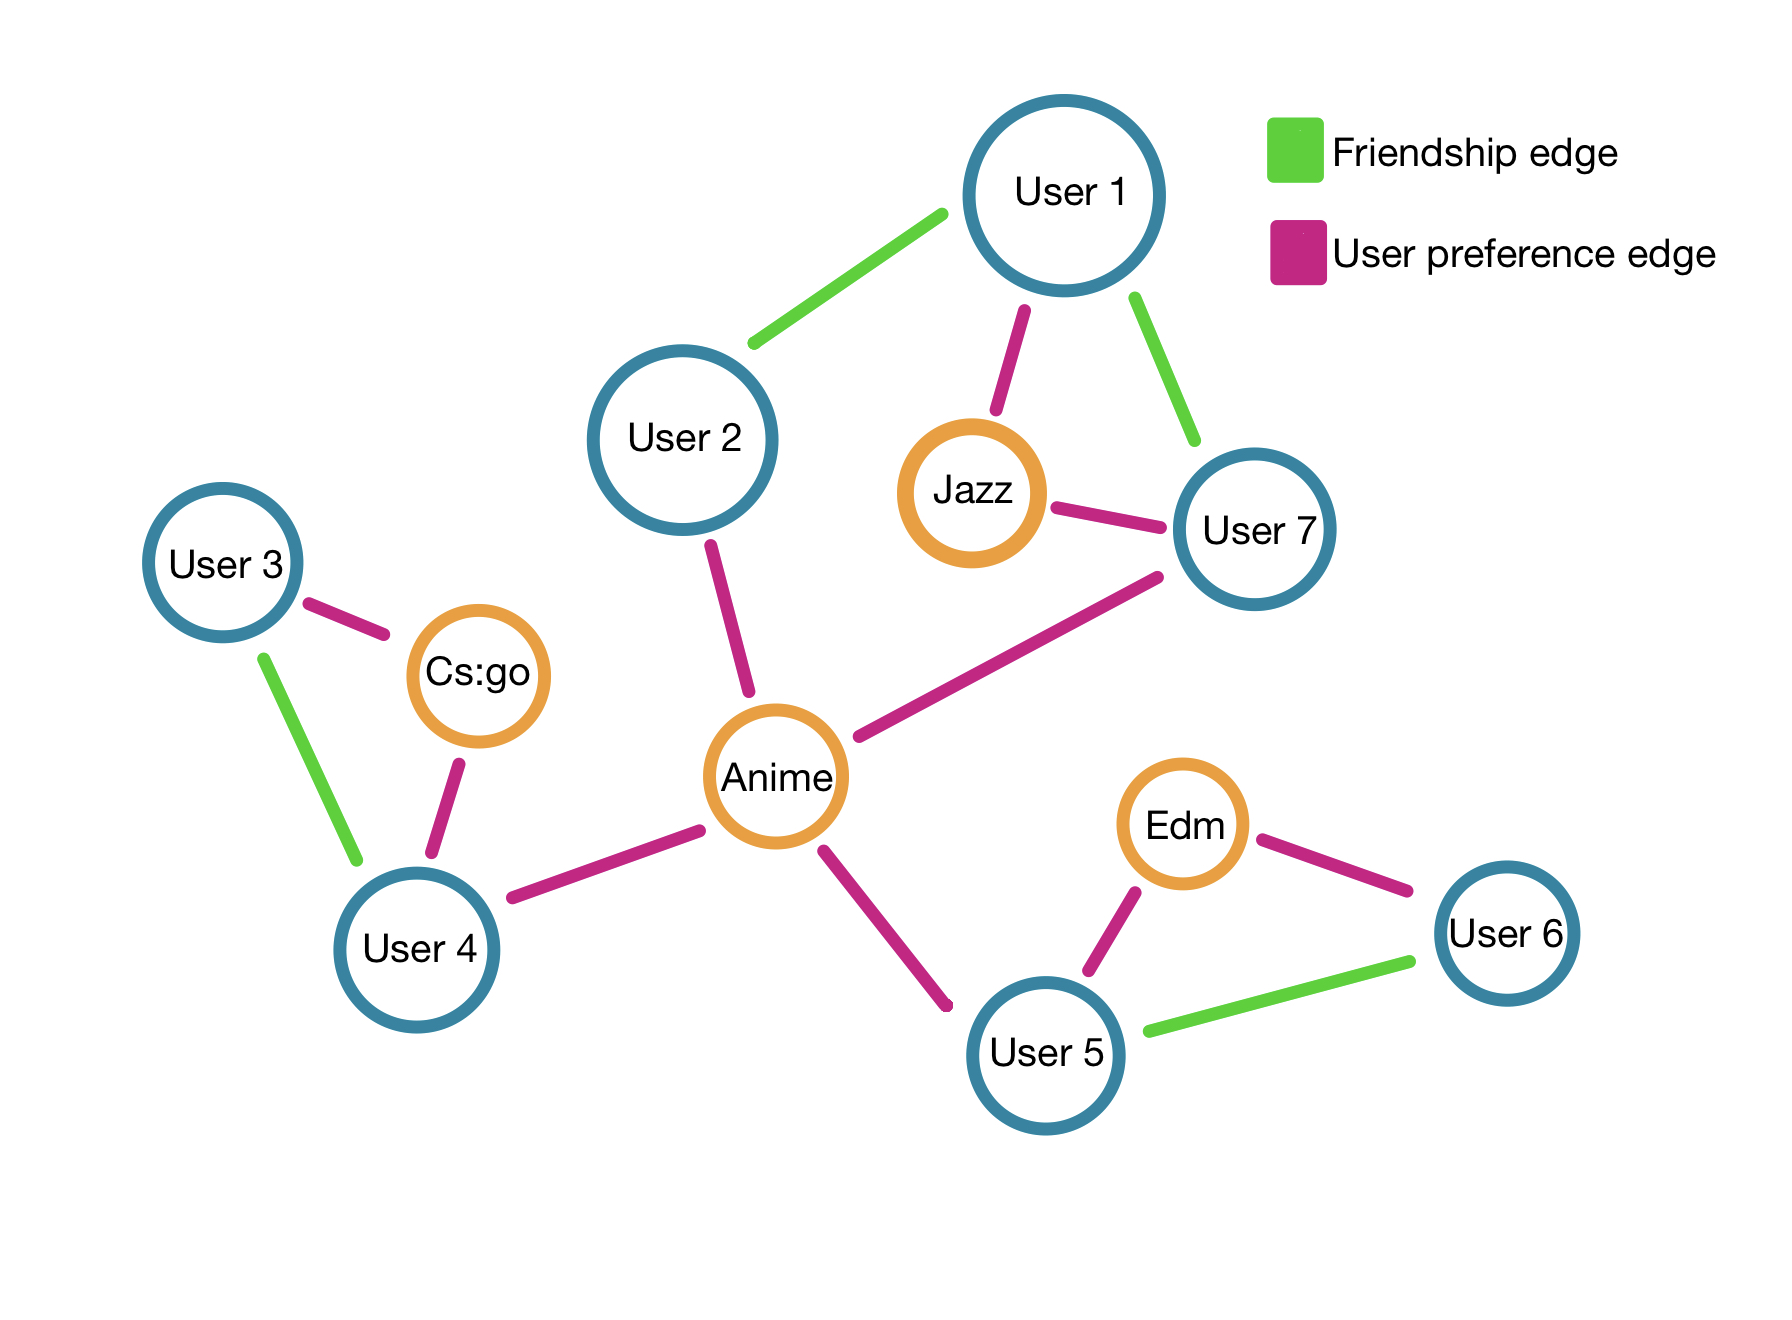
\includegraphics[scale = .2]{Images/graph.jpeg}
\end{itemize}

\newpage 

{\bf Use the Graph to Recommend Friends}

\begin{itemize}
    \item To recommend friends to a user, first we load data for all the users in the database. \\
    
    \item Then we iterate over all the users in the app, using the graph that we built. For each user we calculate a similarity score to the user we want to recommend friends to.\\
    
    \item The similarity score for two users is calculated by calculating the ratio of number of preferences common between the two users and the total number of preferences both users have in total. This score is calculated by \_Vertex.similarity\_score function in recommendation\_graph.py (This part is a bit similar to Assignment 3 but has been modified for our app).\\
    
    \item Let $G = (V, E)$ represent this graph. Let $u_1, u_2 \in V$ represent the two users. Then the similarity score between two users is given by the below formula:
    

     
 \[
  sim(u_1,u_2) = \left\{
     \begin{array}{@{}l@{\thinspace}l}
       \text{0,} & \quad d(u_1) = 0 \text{ and } d(u_2) = 0 \\
       \frac{v | v \in V \text{, v is a preference, } u_1 \text{ and } u_2 \text{ are adjacent to } v}{v | v \in V \text{, v is a preference, } u_1 \text{ or } u_2 \text{ is adjacent to } v} & \quad \text{otherwise}
       
     \end{array}
   \right.
\]~\\

\item The users are then sorted according to their similarity score in reverse order, and we return the top 10 users which had the highest similarity score to the user. \\

\item We also return the similarity score alongside the name of the returned users. \\

\item It is highly unlikely, but a user may not get any friend recommendations with a significant match score. This could only happen when the user does not have many preferences. 
\item The recommendations are returned by the recommend\_friends function in the Graph class in recommendation\_graph.py \\

\item After the recommendations are returned, the user can add those recommendations as friends. 
\end{itemize}

\newpage 

\section{Visualizing friend circle}

The user also would have the feature of visualizing their friend circle. They would be able to visualizing a graph containing their friends, their friends' friends and so on. The graph would be interactive and the user can move the vertices and edges. \\

\begin{center}
    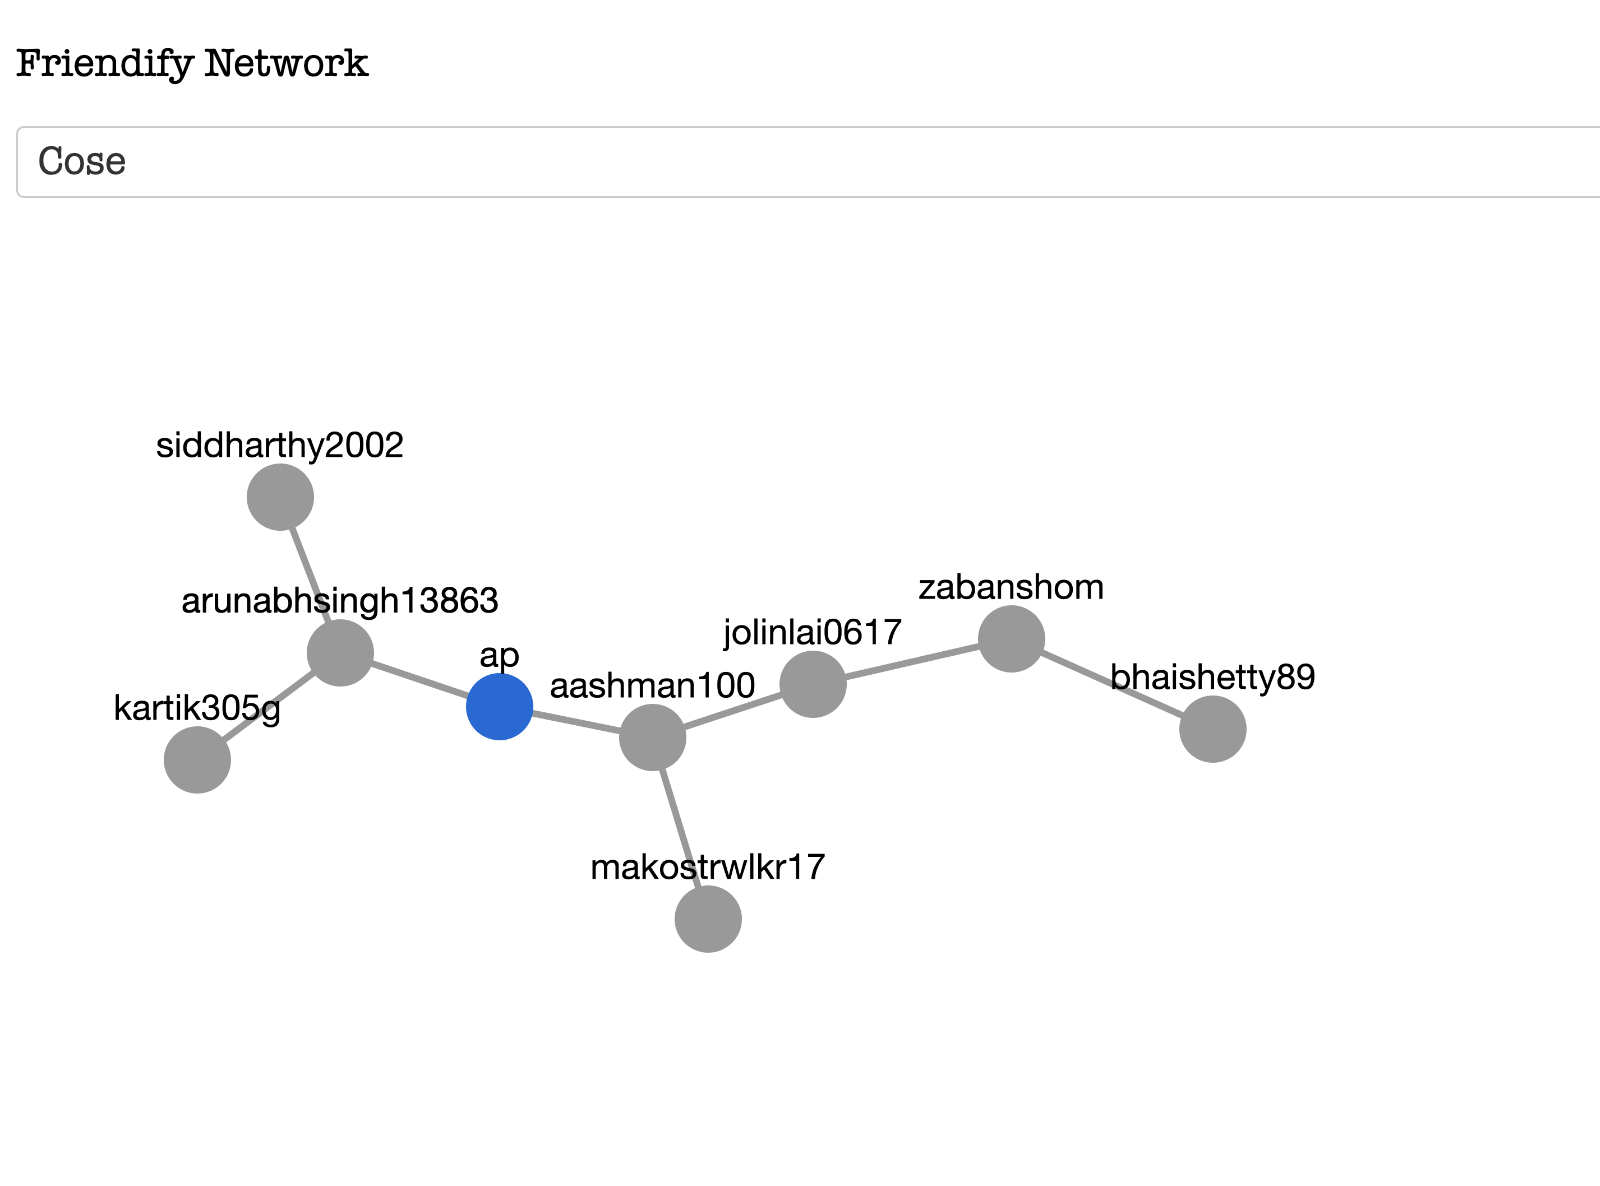
\includegraphics[scale = .3]{Images/graph_ex.png}
\end{center}

We are using Dash for performing this visualisation. Other inbuilt libraries we are using are logging and webbrowser. \\

{\bf Creating the Visualization}

\begin{itemize}
    \item To create the visualisation, we first create the graph using the recommend\_friends function in the Graph class in recommendation\_graph.py.\\
    
    \item Then we recursively create a sub graph of the graph, starting from the user for which we want to create the visualization till a depth d. The depth d represents the depth of the graph. This sub-graph is generated by \_Vertex.generate\_graph function in recommendation\_graph.py. For instance, if the user wants to see only their friends, then the depth would be 1, else if they want to see their friends, and their friends' friends then the depth would be 2 and so on. \\
    
    \item After extracting the sub graph, we again use recursion to format the data for the dash library to plot it as a graph. The formatting is done to make a list of dictionaries representing a vertex or edge. This formated data is generated by \_Vertex.format\_for\_graph function in recommendation\_graph.py \\
    
    \item After getting the formatted data, we use the Dash library, to visualize the network. Specifically we plot a Cytoscape graph. We have also used Dash's DOM objects to add the feature of representing the graph in different ways, including 'breadthfirst', 'grid', 'random', 'circle', 'cose', and 'concentric'. The ploting is done in the plot function in Graph class in recommendation\_graph.py\\
    
    \item The graph does not open automatically, so we used the webbrowser library, which is an in-built library, to open the site where the visualisations are happening. We have set the app to run on localhost 5050. \\
    
    \item All the verties and edges in the visualized graph are interactive and can be moved around. 
\end{itemize}




\section{Searching for People}

The user also has the feature to search for people by their user ID. This is similar to what can be seen on social media apps. \\

This feature returns the top search results, which are the most similar user IDs to the search query, which the user typed in. \\

The user can then go into the profile of the search results, and add them as friends, or unfriend them if they are already friends.~\\

{\bf Process of Searching a Query}

\begin{itemize}
    \item First we load up all the user IDs we have in our app's data from the firebase database.\\
    
    \item We then pass the list of user ID's into the merge sort algorithm, but with an extra argument that is the search queue to which the user IDs are being compared. The sorting algorithm is in the SearchPeople class in screen.py\\
    
    \item To get the similarity score, we are using a class from an inbuilt library called difflib, which is SequenceMatcher. The score is calculated in the function similar in the SearchPeople class in screen.py\\
    
    This class takes in an argument two sequences. We access the ratio function of the SequenceMatcher, which returns the similarity ratiop between the two sequences (in our case which are the user IDs).\\
    
    \item We use this similarity between the query and the user IDs as the key to sort and get the top search results. \\
    
    \item We are returning only the top 10 search results, which have the highest similarity to the search query.
    
    \item The user can now go into the profile of the search results, and add them as friends, or unfriend them if they are already friends
\end{itemize}

\newpage 

\section{User Interface handling}

Friendify is a terminal app, and we have intensely used Object Oriented Programming to create the view control of the app. \\

The app is divided into different screens, for instance home screen, sign in screen, registration screen and many more. \\

Each screen shown in the app is represented as a Screen object. Each type of Screen has its own class which inherits from the Screen class, and is responsible for keeping track of its view, and deciding what needs to be shown next, that is which screen to show next. \\

For instance, the HomeScreen inherits from Screen object and is responsible for representing a home screen, similarly there is DocumentationScreen which is responsible for showing any arbitrary document or string as a document. \\

All the Screen classes are contained in the screen.py file.\\

{\bf Transition between Screens}

\begin{itemize}
    \item Each Screen object inherits a show function. This function is responsible for printing the content of the screen and handling the transition to the next screen. \\
    
    \item The show function always returns a Screen object, which represents the next screen to show. this is how we transition from one screen to another.\\
    
    \item As the app starts running, the current screen is set to the HomeScreen and a loop is set to:
    
    
    \begin{minted}{python}
    current_screen = HomeScreen()
    
    while current_screen:
        current_screen = current_screen.show()
    \end{minted}
    
    
    This loop transitions from one screen to the another, but if the current screen is None then the app would stop. This would only happen when the user wants to exit the app.  
    
    
    \item To decide which is the next screen to transition to, the show function uses Pyinquirer and cuti, both of which are used to inquire in the python terminal in a beautiful way. Both of them have wide variety of questions we can ask.\\
    
    \item Our program passes a list of questions to Pyinquirer or cuti, about where the user wants to navigate, and they intern ask the question in terminal in an interactive way, and return the answer to our program.\\
    
    \item These questions are either hard-coded in constants.py file or can be created from the generate\_question\_with\_choices and generate\_question\_multi\_choice functions in the constants.py file. \\
    
    \item The program the returns the appropriate screen according the returned answer.
\end{itemize}~\\

Different Screen objects also contain functions to perform their own computations. For instance the SearchForPeople Screen, screen which searches for query, have a merge sort function which helps in giving the top search results. \\\\

{\bf Operating Systems}~\\

Our app intensively uses terminal commands to make the screen interactive. For instance every time the app transitions from one screen to another, we clear the screen. \\

But, the terminal apps for windows, mac and linux are different and take in different commands for the same task. For instance to clear the screen of the terminal mac and linux use clear command but windows uses cls command. \\

We have used python's inbuit library called sys, which has an attribute called platform which returns different values for different operating systems. For instance for mac it return darwin. \\

We are using this attribute to distinguish between the different systems and use the system specific commands. These are used in Screen.clear\_screen function in screen.py and constants.py file. \\

We even have different messages for different operating systems, as windows operating system does not support emojis and many special characters. This can be seen in constants.py file.\\\\

{\bf Logo }\\

We are also using pyfiglet library to print beautiful terminal logo for our app. pyfiglet returns a string representation of a piece of text in ASCII characters. The function to print the logo is print\_logo in the constants.py file.

\newpage 

\chapter{Download/Obtain Datasets} 


Initially  our  app  would  not  have  any  registered users. \\

Thus, we conducted a survey and registered 50 users with our app. \\

This data is stored in the firebase cloud.\\

This data set is NOT used while running the app. \\

 We have still provided the {\bf dataset as a zip file (data.zip)} with our submissions, although it is  {\bf  not required to run the app.} \\
 
 The dataset was located in a folder named "data". so the path to the dataset is "data/Survey.csv"
 

\chapter{Running the App}

\textbf{Apart from the instructions provided below, we had made two videos (one for mac and one for windows) on how to use our app.}\\ 
\textbf{We recommend {\Large watching the VIDEOS first} and then reading the instructions (provided below).}

\begin{enumerate}
    \item First download all of the requirements from requirements.txt
    
    \item Note that this is a terminal app and would \textbf{ONLY work in the terminal (and not on python console)}. Open the app in Pycharm and click on the terminal icon on bottom left of the Pycharm screen. 
    
    \begin{center}
        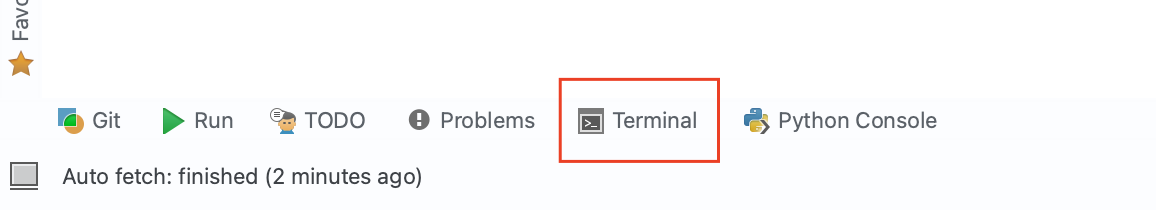
\includegraphics[scale = .5]{Images/terminal_icon_2.png}
    \end{center}
    
    \item Type "python main.py" in the terminal. \textbf{Note that this line could change from system to system. If this does not work you can try "py main.py" or "python3 main.py".}
    
    \item As soon as the line is run in the terminal, the app should start running and this is how the screen should look like: 
    
    \begin{center}
        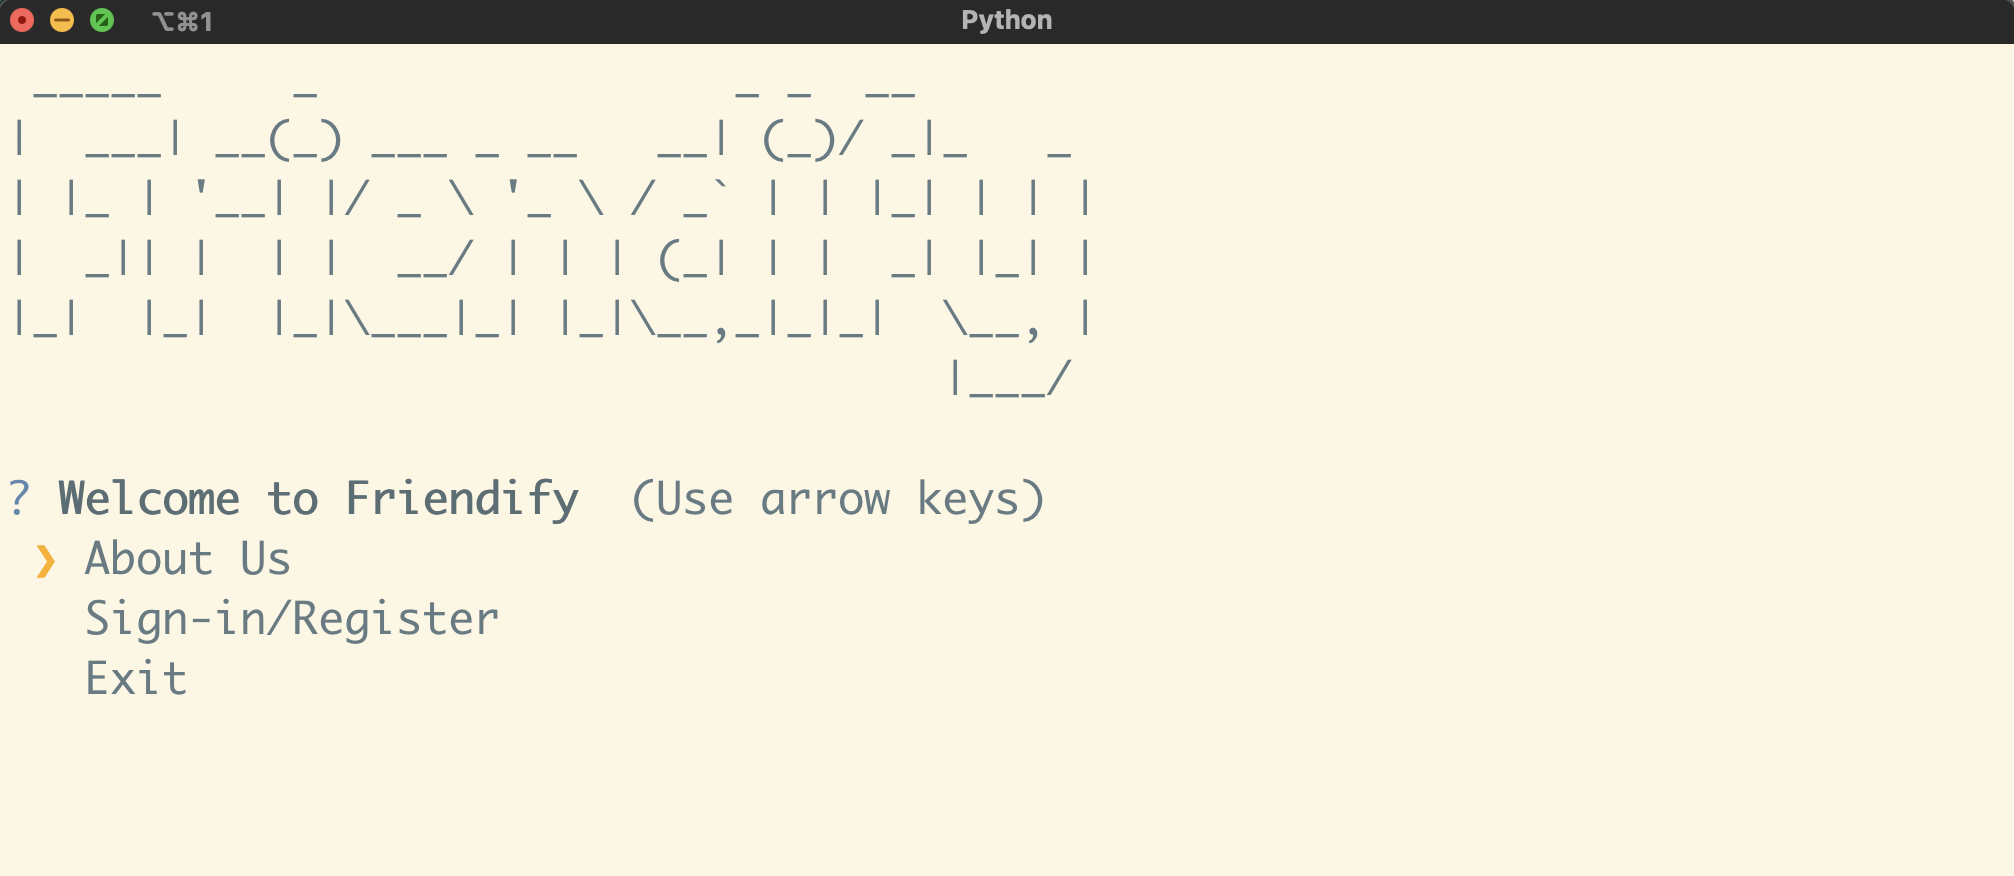
\includegraphics[scale = .35]{Images/home.png}
    \end{center}\\

    This is the Welcome Screen of our app. On the Welcome Screen the user will get 3 options
    
    \begin{itemize}
        \item About us - which consists of information about the app
        \item Sign in or register - which is used to sign in or register to the app
        \item Exit the app
    \end{itemize}
    
    \item Now using arrow keys, go to the Sign-In/Register option and press enter. Now the screen should change and should look something like this:
    
    \begin{center}
        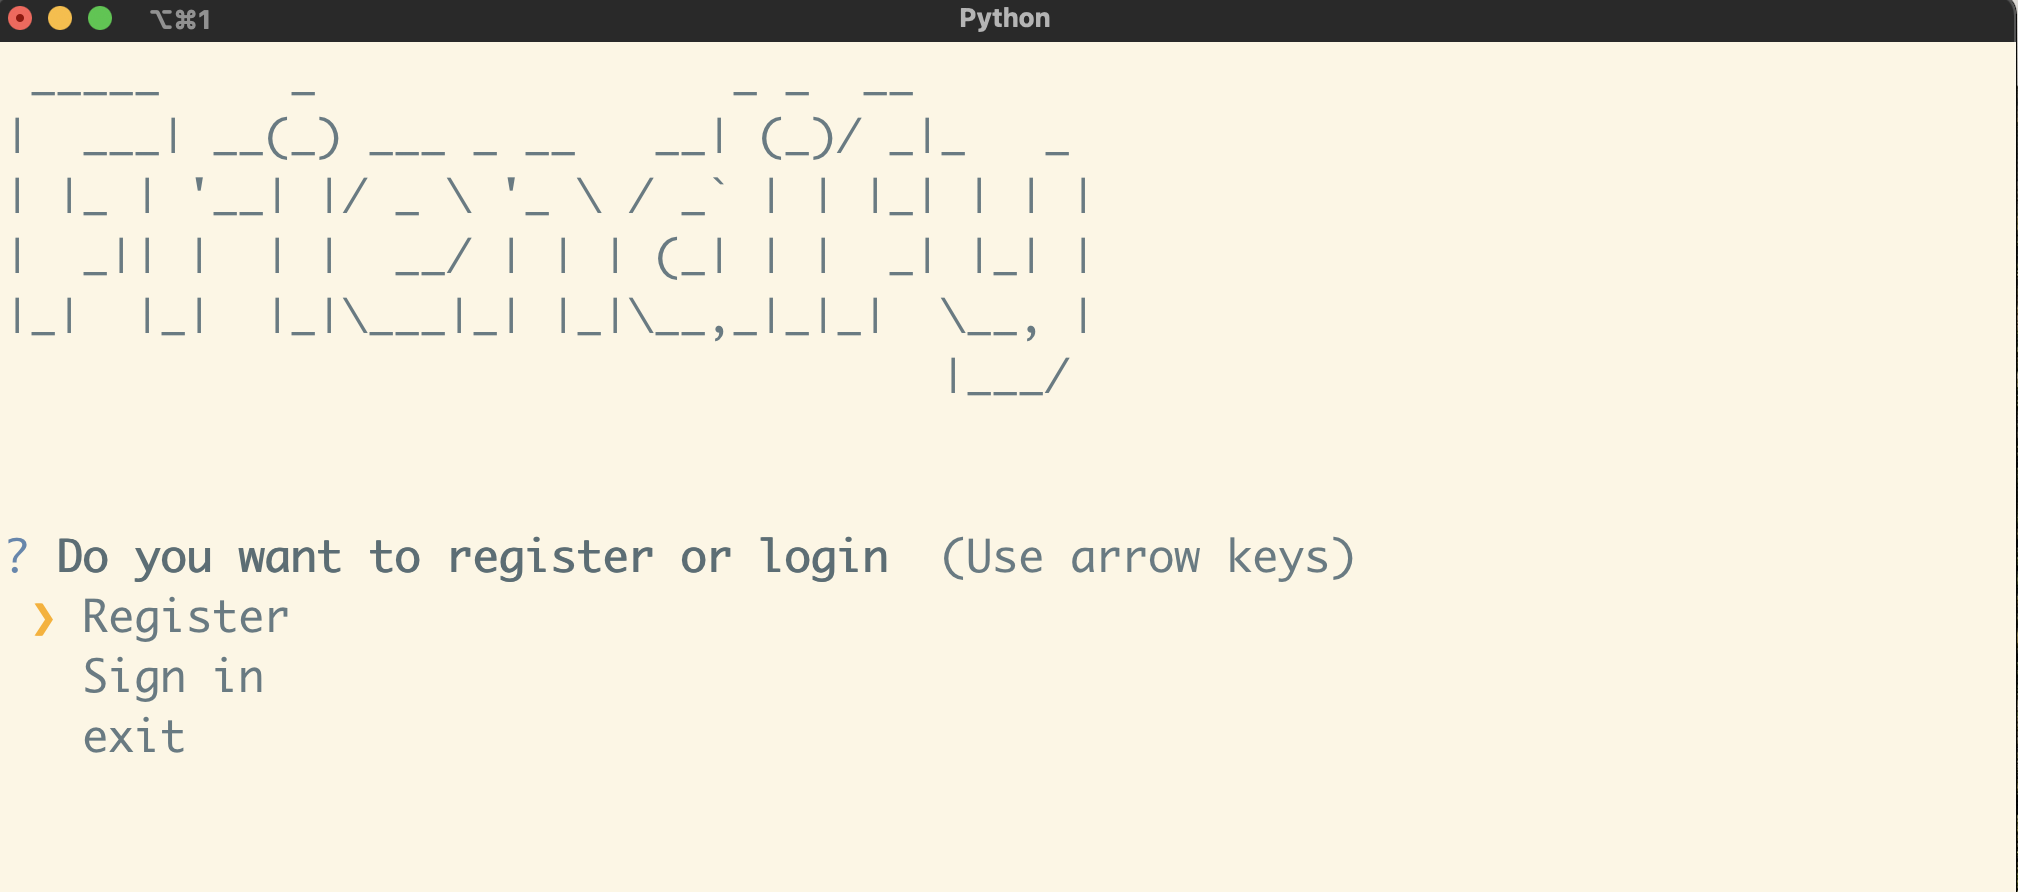
\includegraphics[scale = .31]{Images/sign_in_register.png}
    \end{center}
    
    
    \item Now, navigate to register if you are not signed up and otherwise go to Sign in. \\
    
    
    {\bf \underline{{\Large If you clicked Register}}}
    
     \begin{enumerate}
         \item If you clicked register, you will be asked to enter a username. This username would be unique to you. This is how the screen should look like:
         
           \begin{center}
             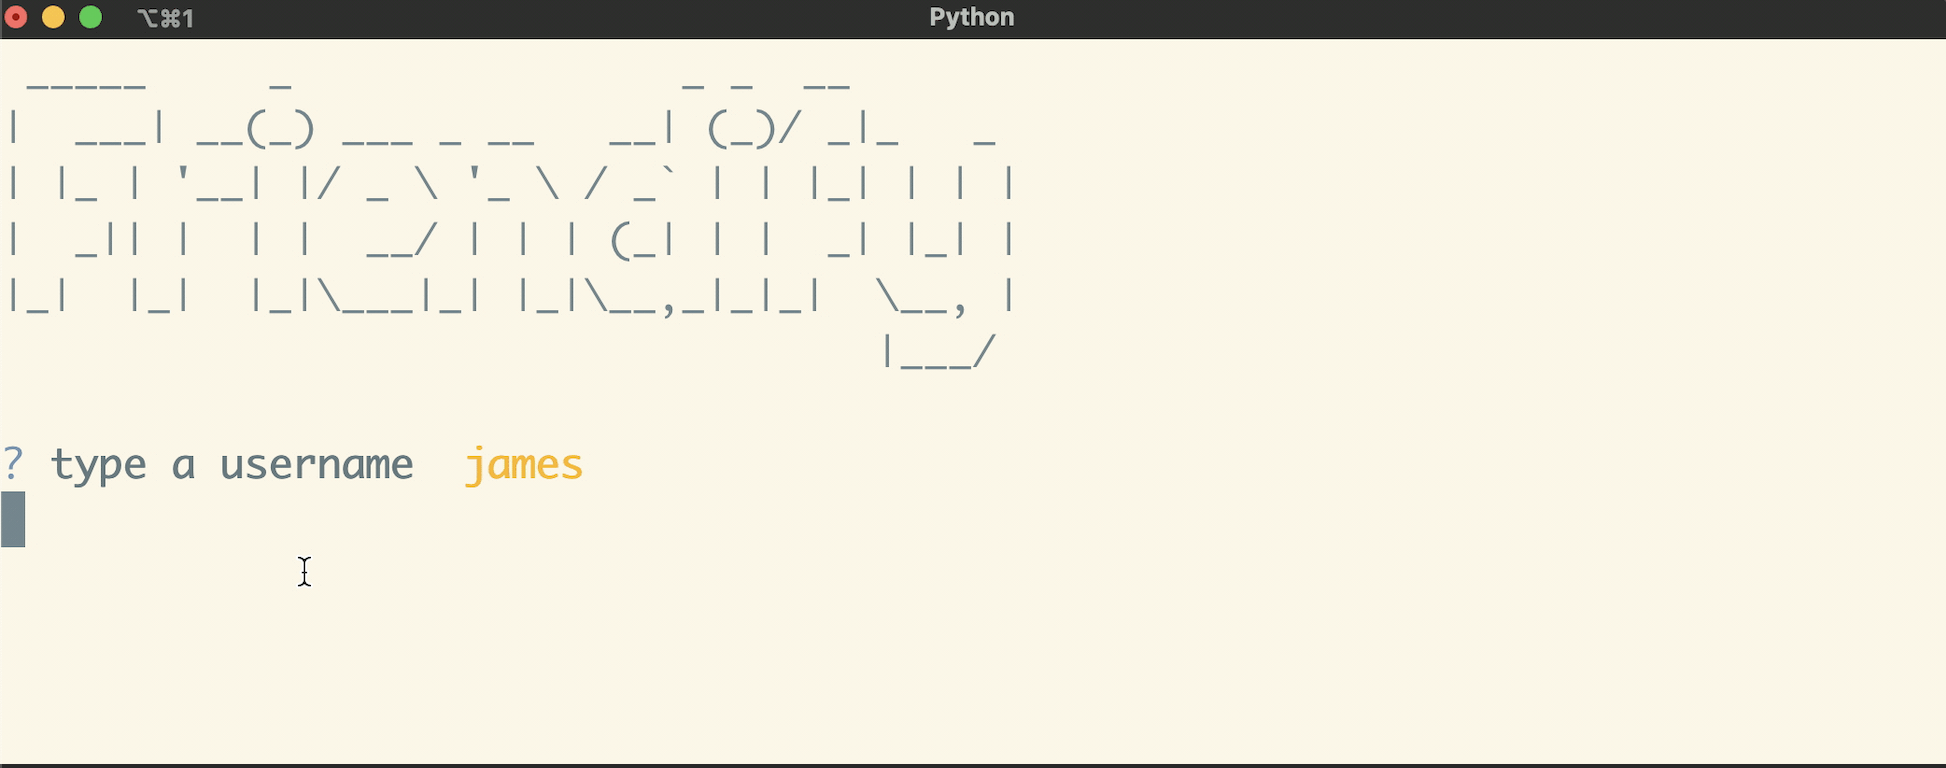
\includegraphics[scale = .25]{Images/register-name-q.png}
            \end{center}
            
        \item After entering your username, 4 other questions would be asked about your preferences - movies, music, games and the food you like. This is how one of them should look like:- [\textbf{ You can move up and down using the arrow keys and select an option using the space-bar}]
        
        \begin{center}
             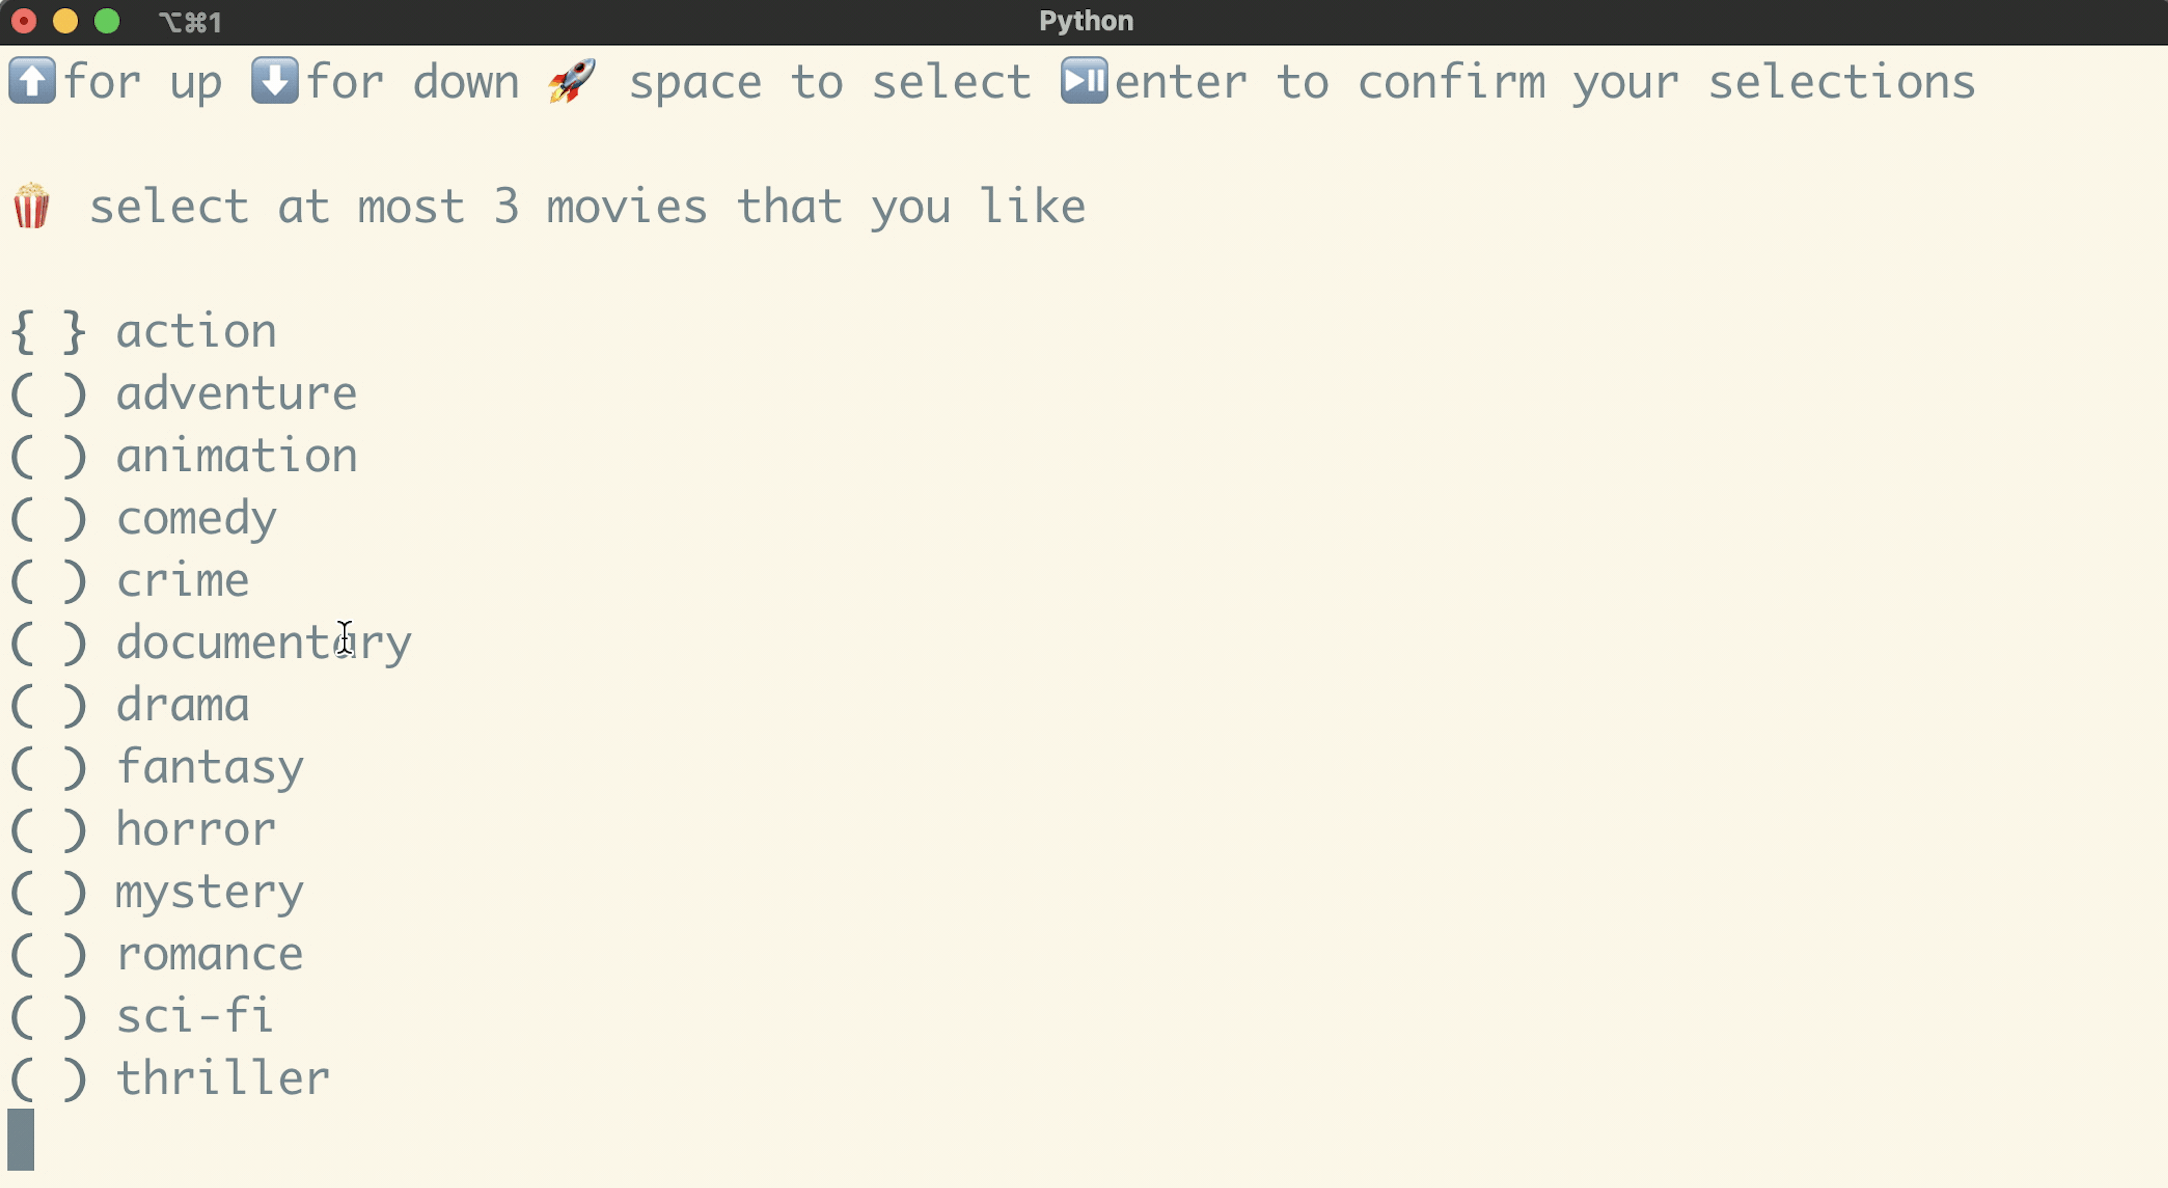
\includegraphics[scale = .25]{Images/register-other.png}
            \end{center}
        
     \end{enumerate}
     
     {\bf \underline{\Large If you clicked Sign In}}
     
     If you clicked sign in, you would only be asked to type the username with which you registered. This is similar to when you are asked to fill in a new username while registering. this is how it should look: 
     
      \begin{center}
             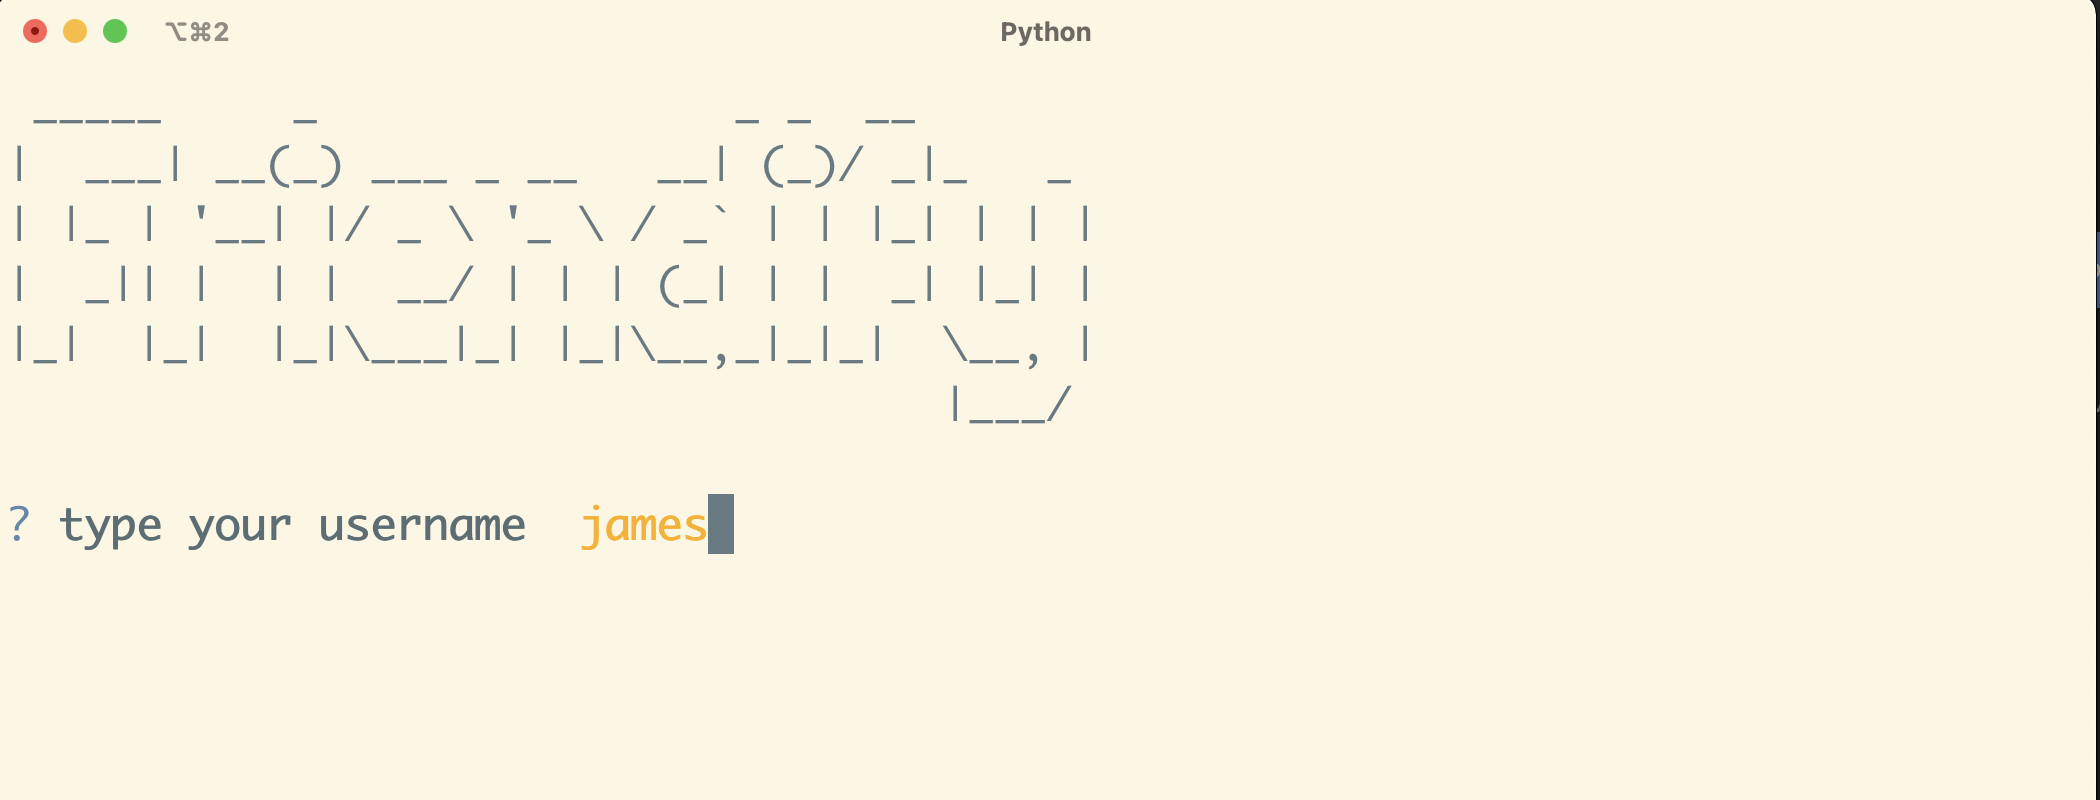
\includegraphics[scale = .3]{Images/sign-in.png}
      \end{center}~\\
    
    
    {\bf After Answering the Registration/Sign-In Questions} you would be navigated to your home screen \\
    
    \item Now you should have entered your home screen, and this is how it should look like: 
    
     \begin{center}
             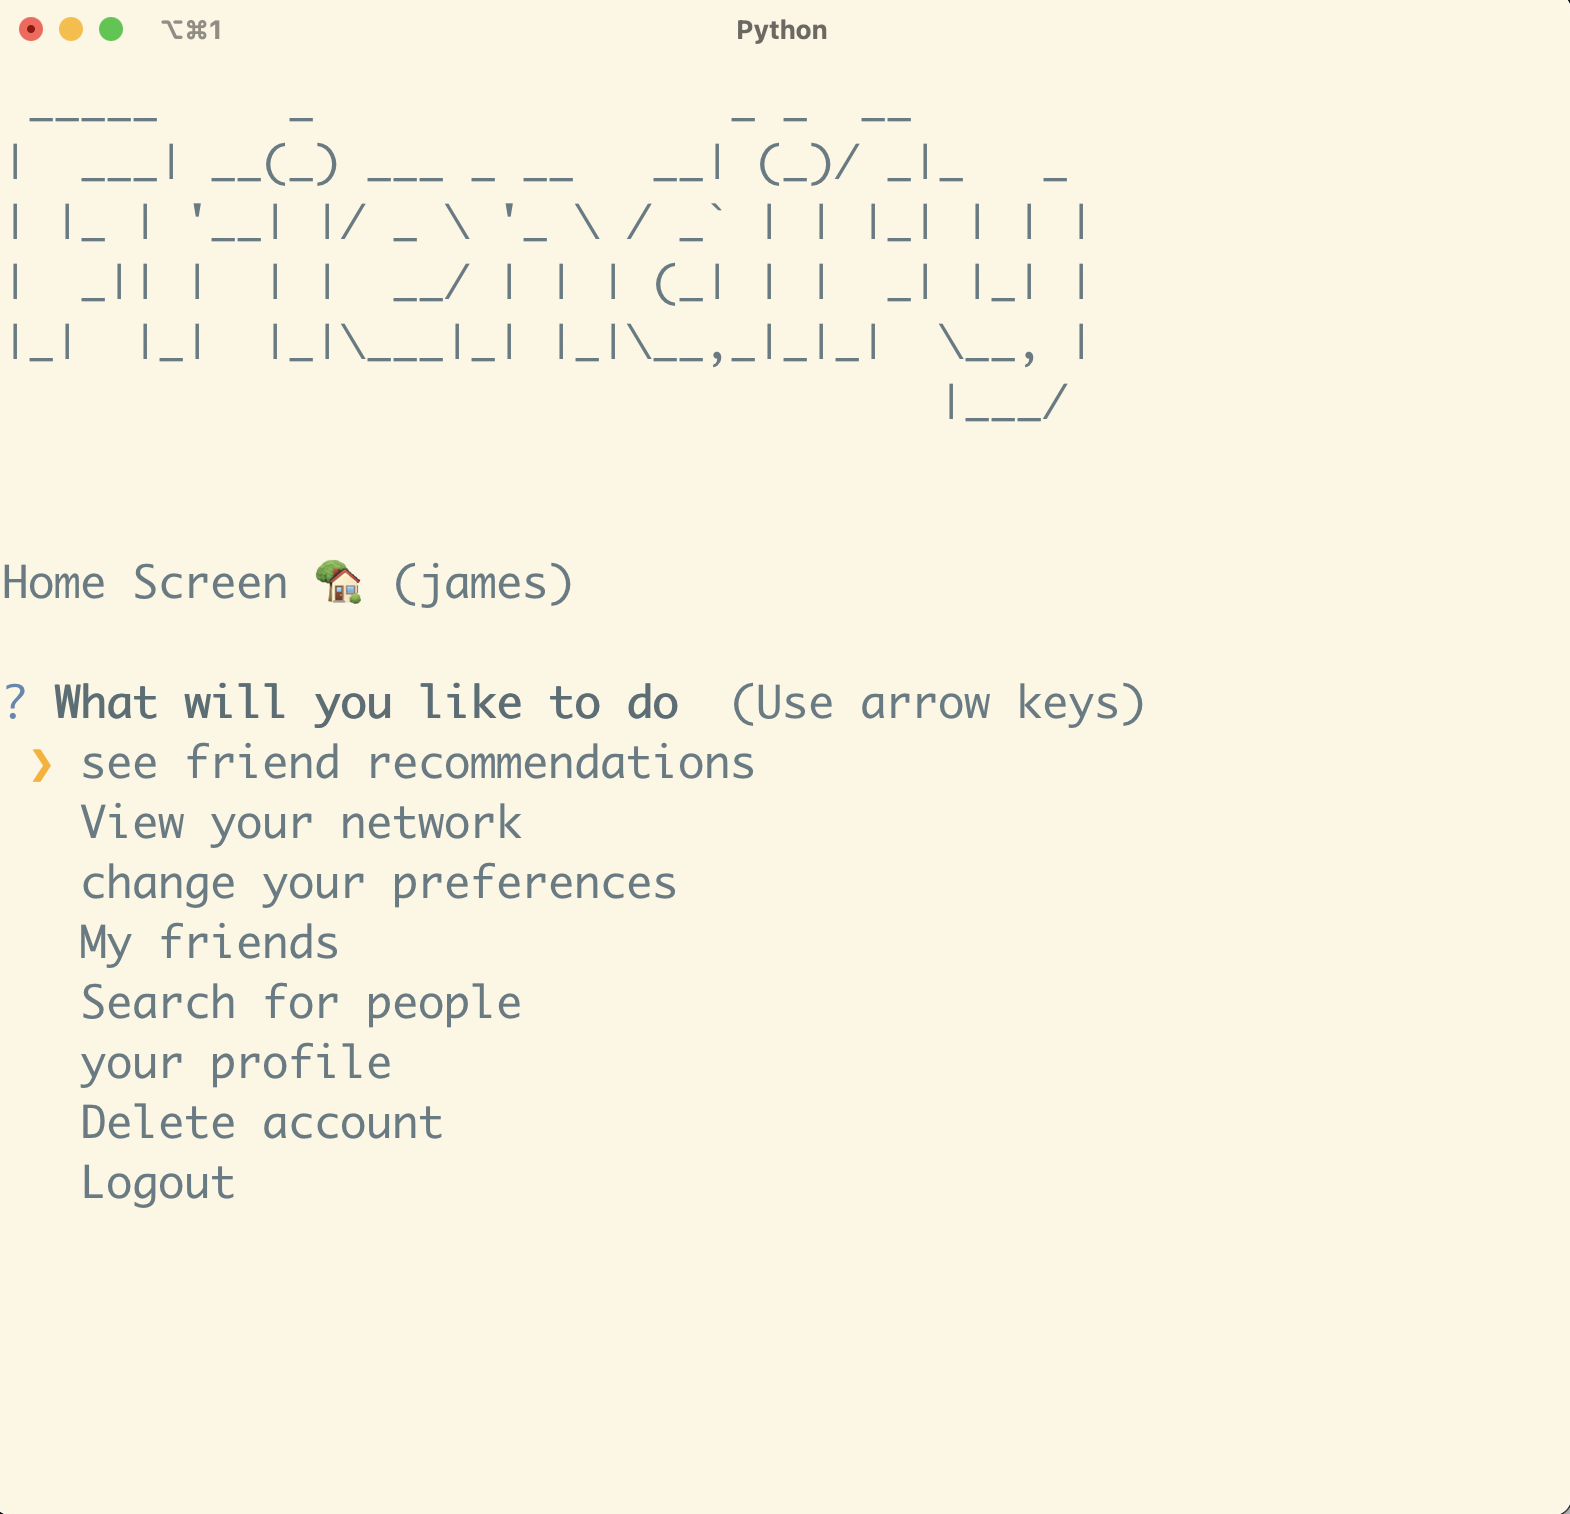
\includegraphics[scale = .45]{Images/signedin100.png}
      \end{center}~\\
      
      Form your home screen you can:
      
      \begin{enumerate}
          \item {\bf see friend recommendations } : navigates you to your friend recommendations. After navigating, you should see a screen which looks like this: 
          
          \begin{center}
             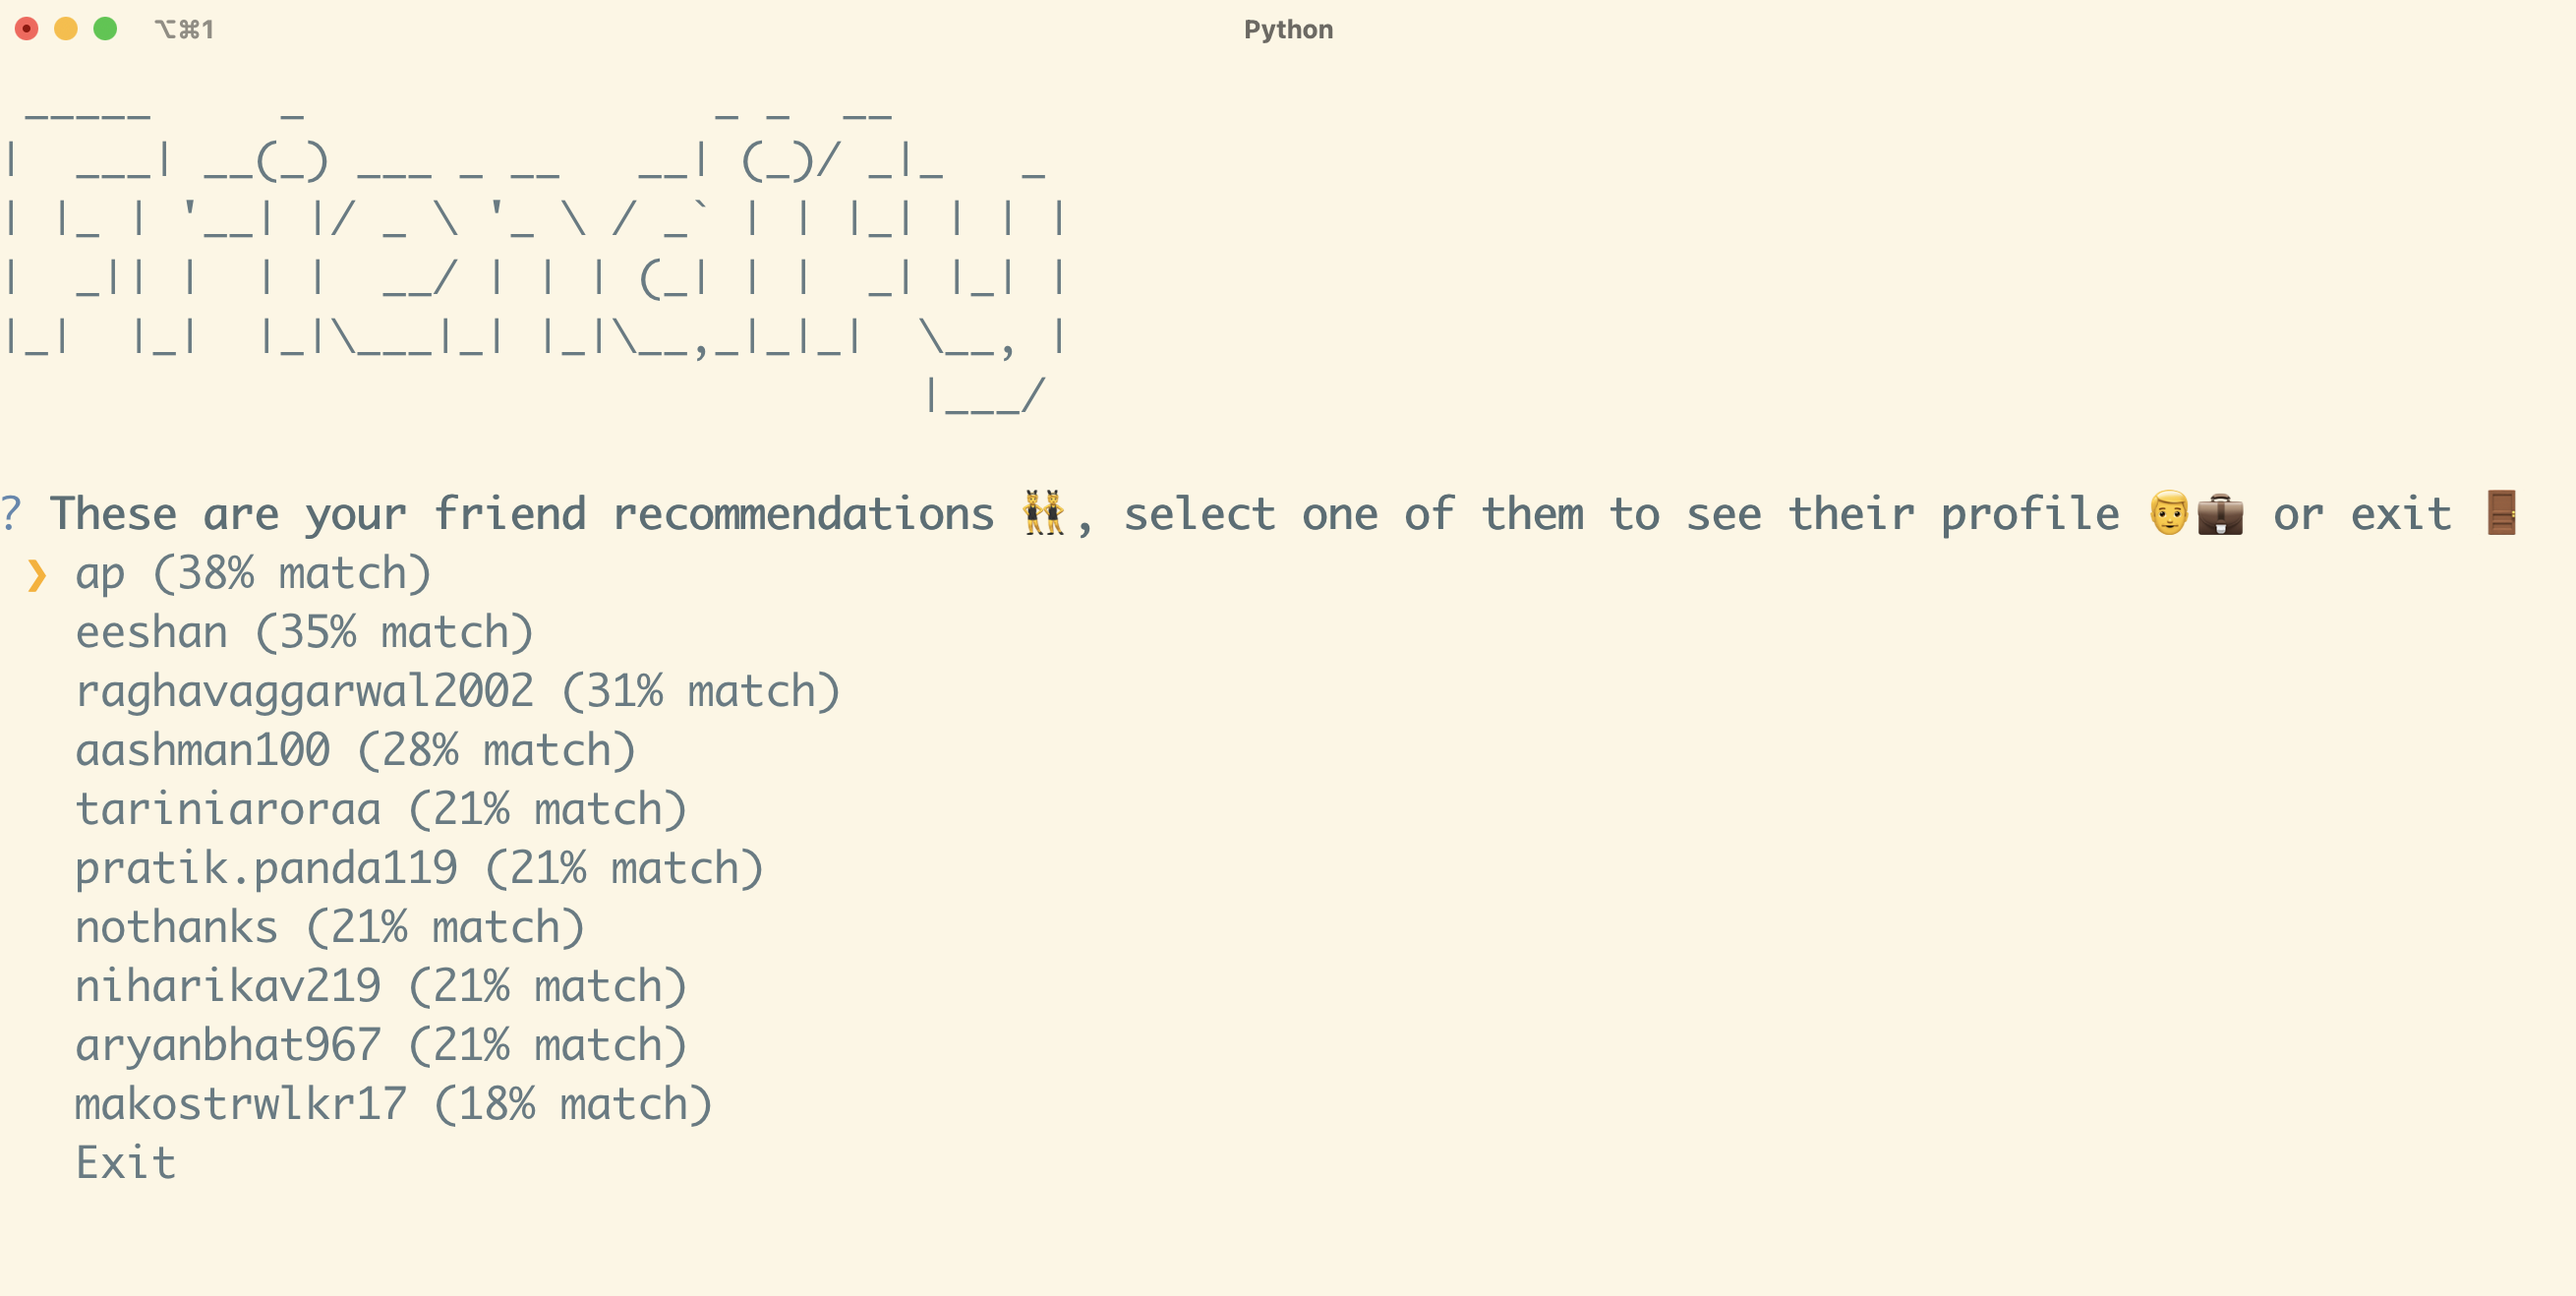
\includegraphics[scale = .3]{Images/recc100.png}
      \end{center}
      
      For here you can navigate to any of the users listed below, and this is what you should see:
      
      \begin{center}
             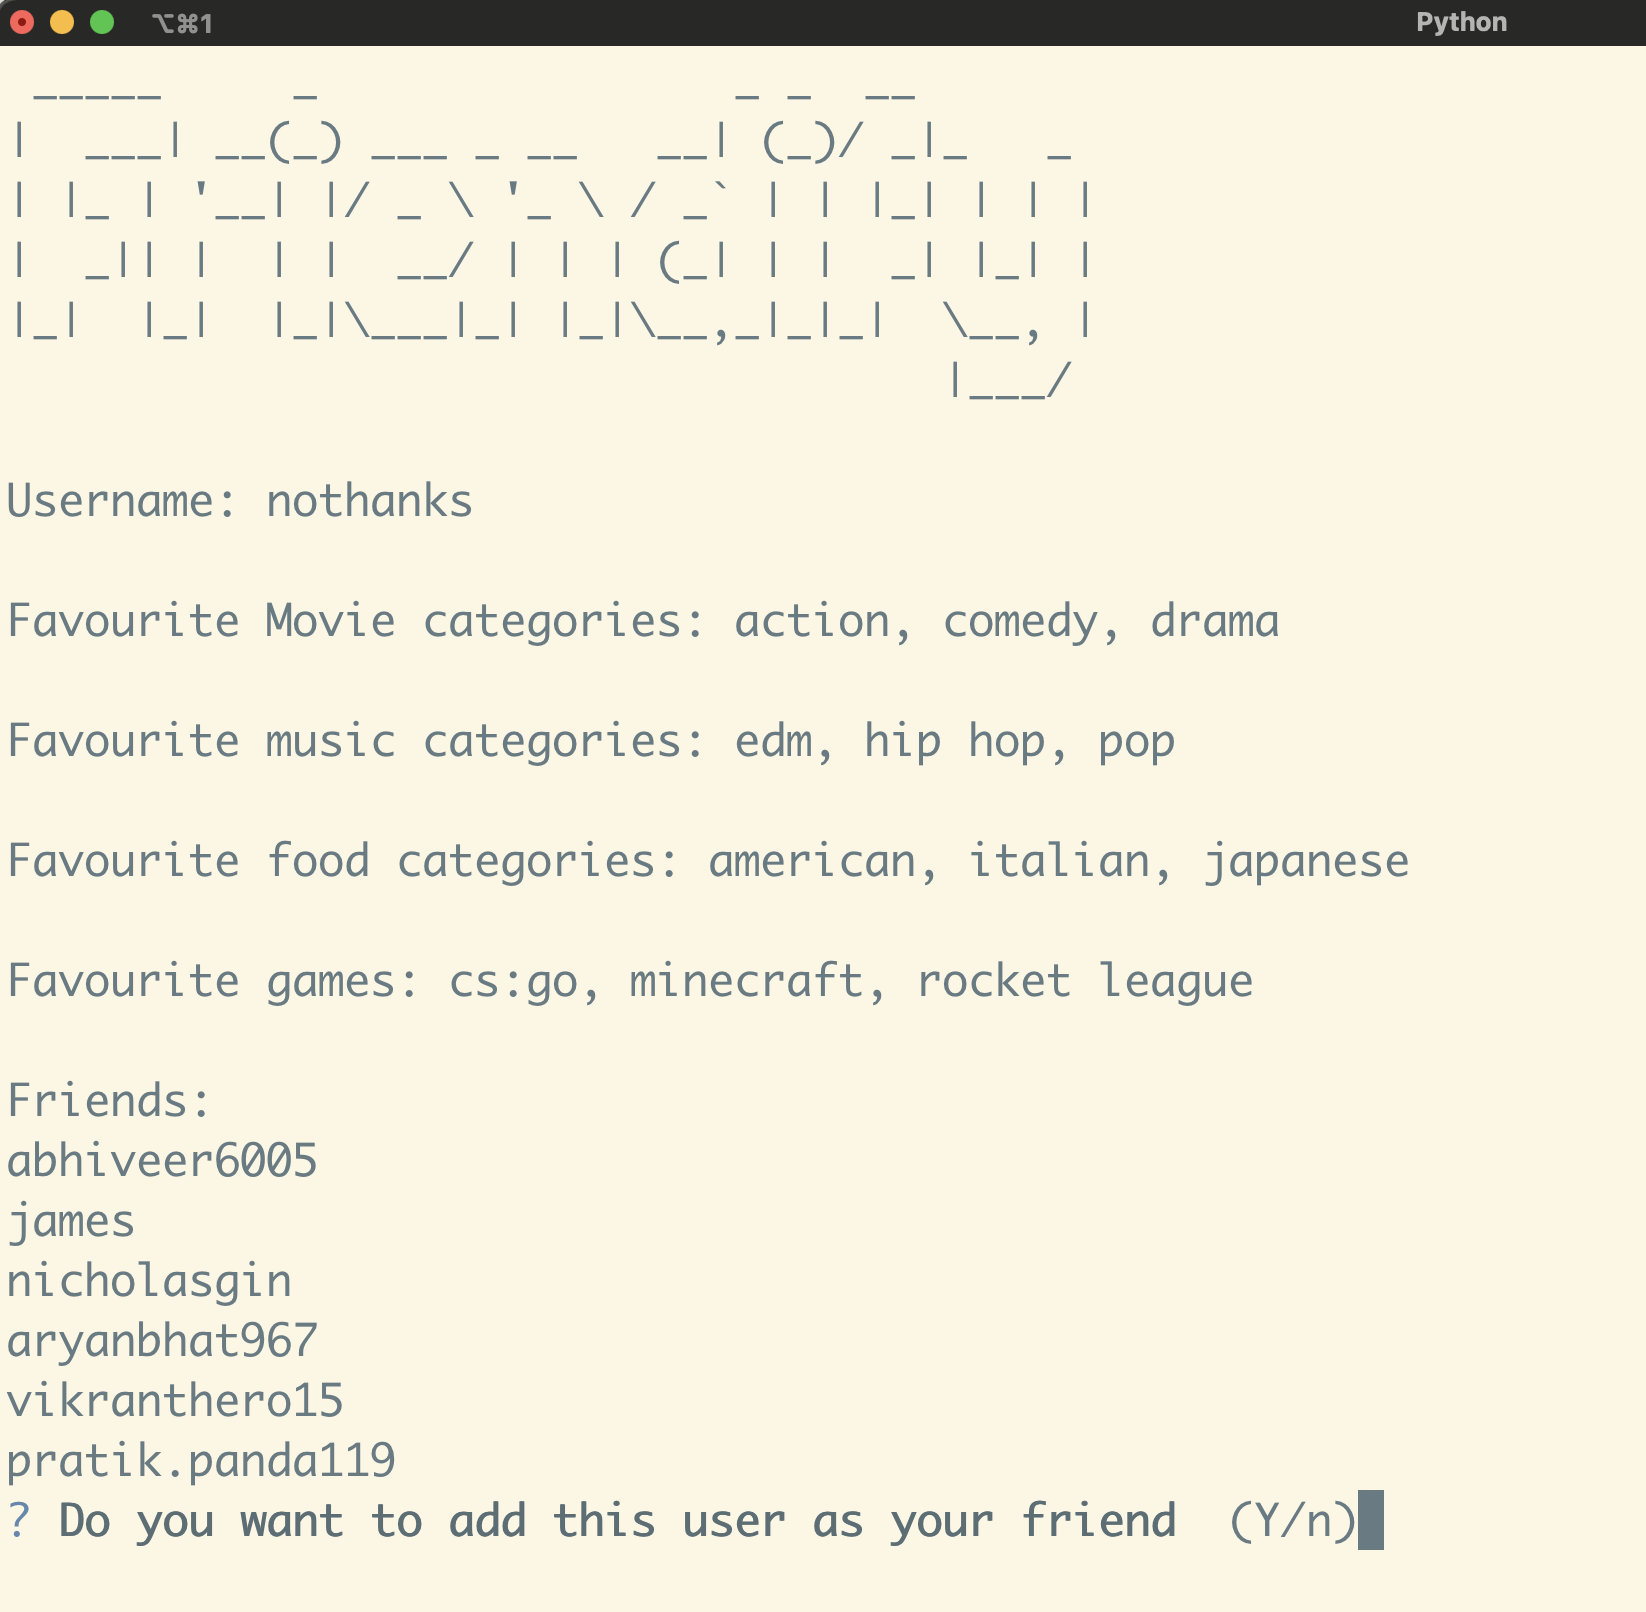
\includegraphics[scale = .3]{Images/user_profile_rec.png}
      \end{center}
      
      This is the user's profile, which contains all the information about the user. You have the option to add them as your friend. After choosing whether you want to friend the user, you would be navigated to the previous screen containing you recommendations.
      
      \item {\bf View your network} : This option is used to visualise your friend circle. The option would navigate you to the following screen:
      
      \begin{center}
             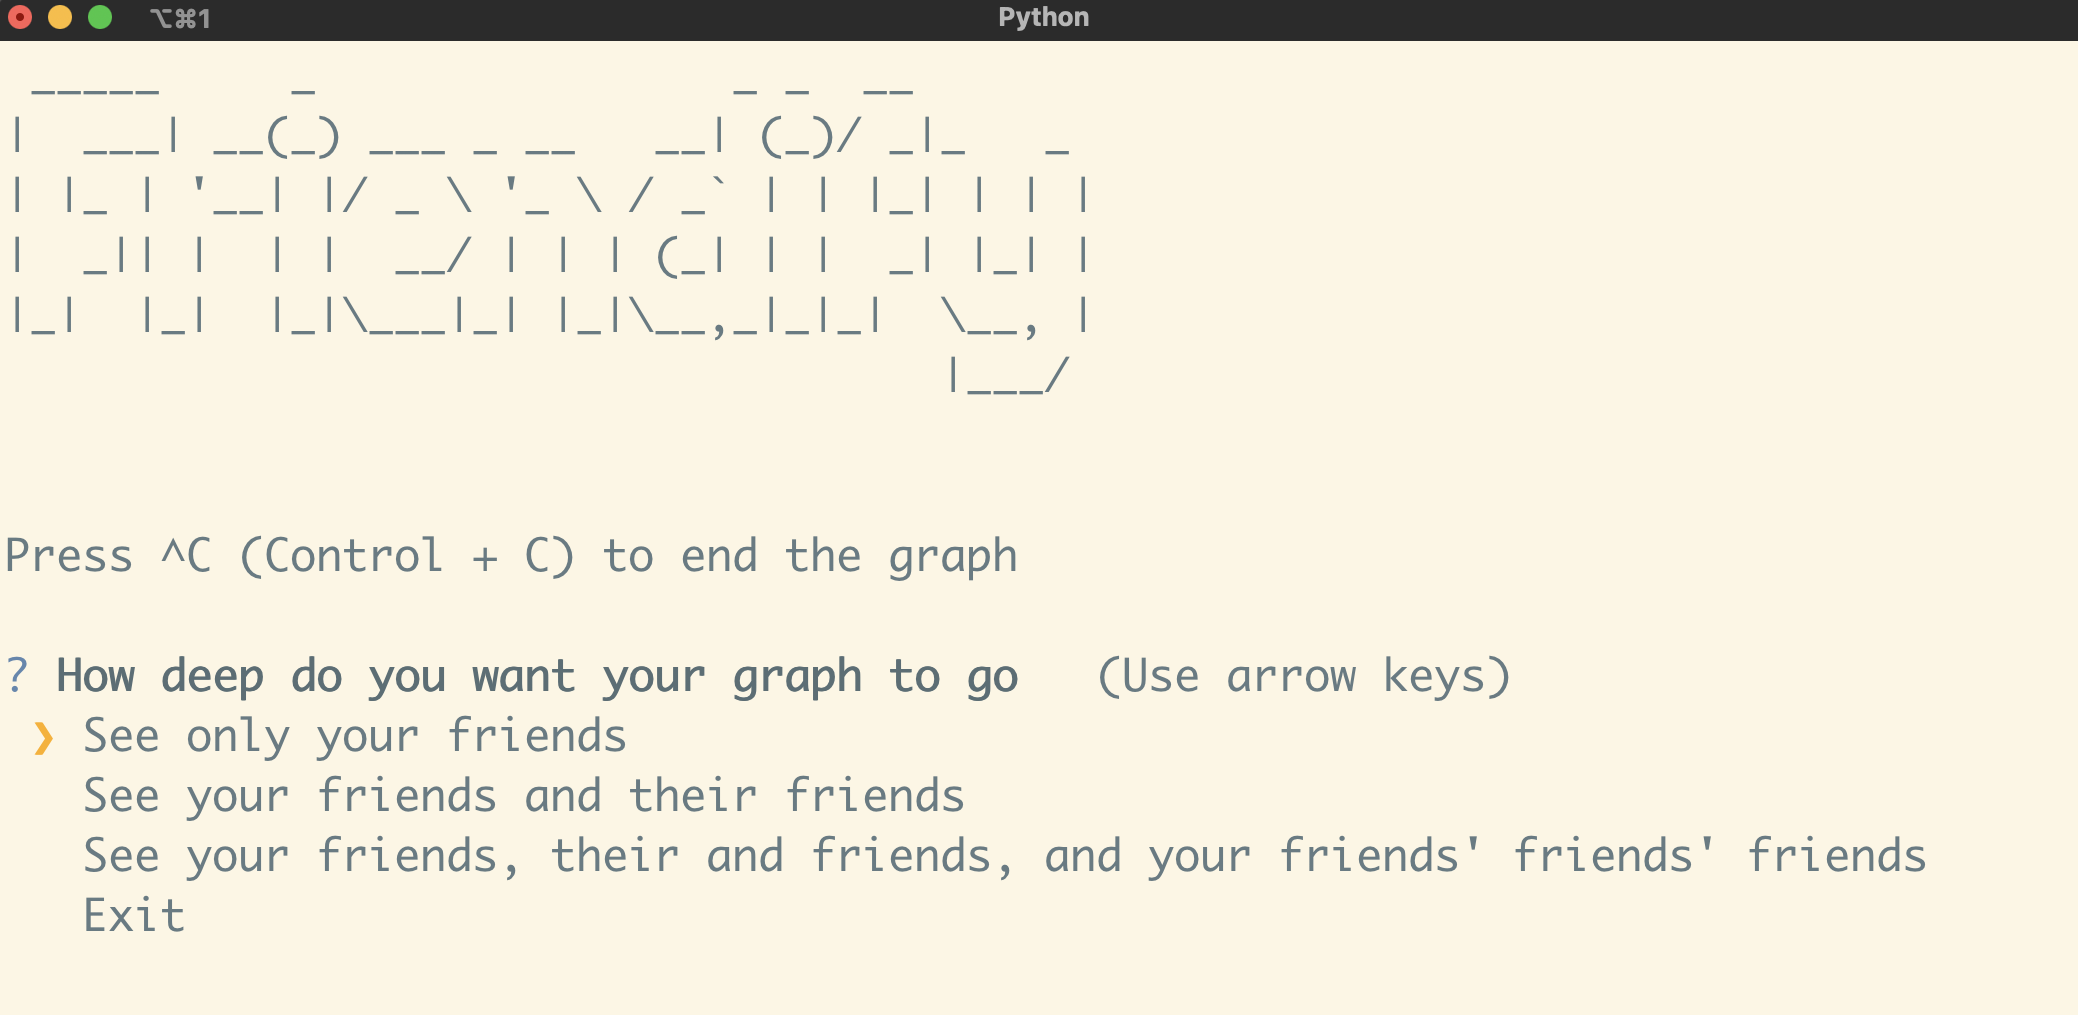
\includegraphics[scale = .35]{Images/graph_depth.png}
      \end{center}
      
      From here you can choose from the three options, of seeing only your friends, or your friend and their friends or or your friend, their friends, and their friends. \\
      
      After selecting an option, you would automatically be navigated to a web-browser. If you are not just enter http://127.0.0.1:5050/ in your web-browser. \\
      
      After viewing your visualisation in the browser, you can come back to the app. This is how it should look:
      
      \begin{center}
             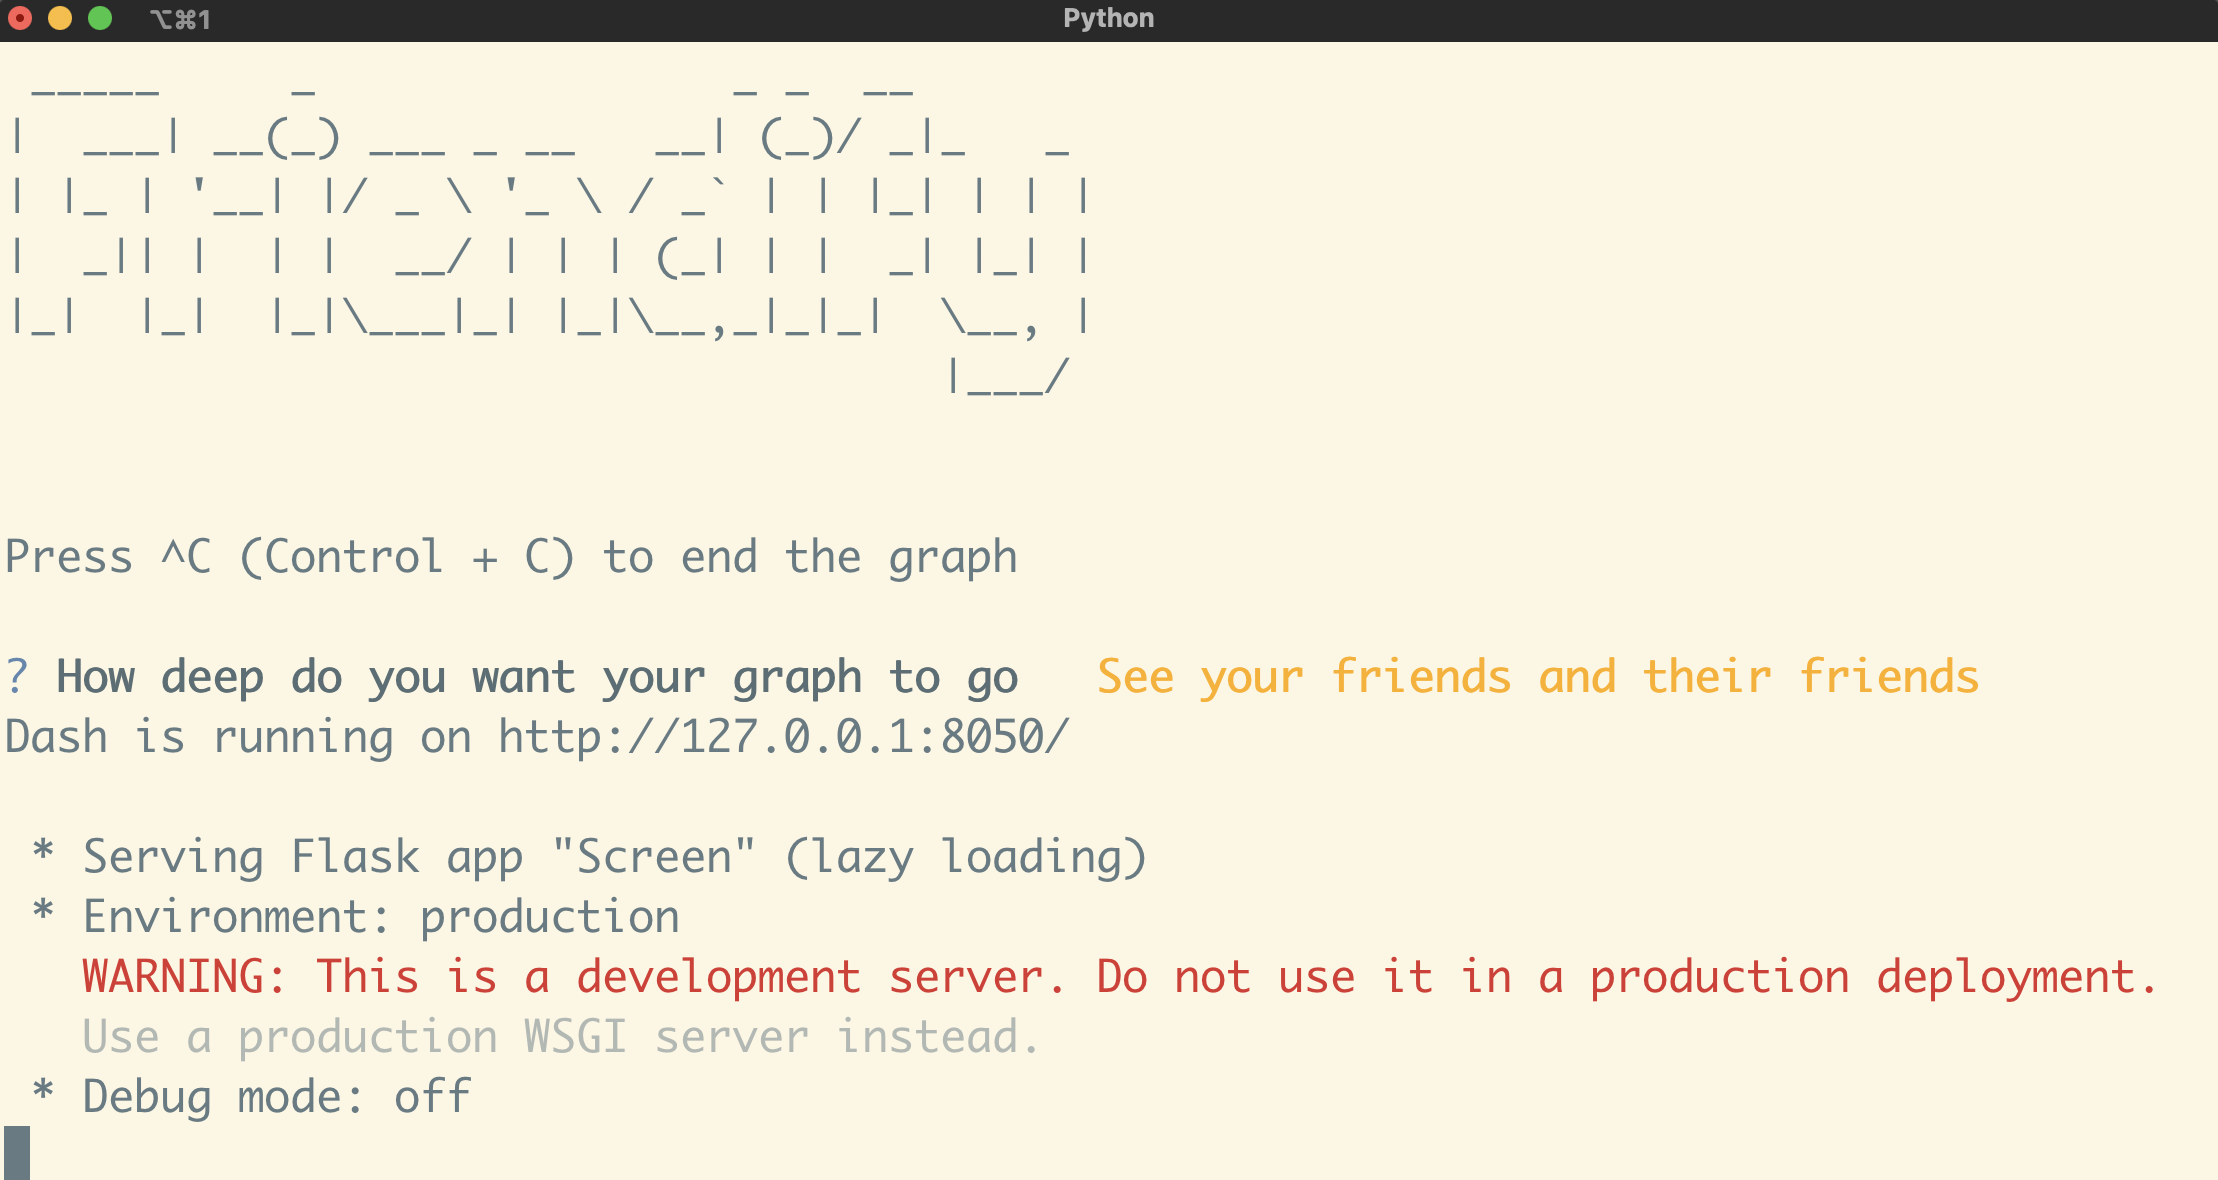
\includegraphics[scale = .3]{Images/graph_init_2.png}
      \end{center}
      
      End the visualisation by pressing Command + C (on windows) or Control + C (for mac).After you exit this screen, you would be navigated to the home screen.\\\\
      
      \item {\bf change your preferences} : this feature is used to change the preferences you choose during registration.
      
      
      \item {\bf My Friends} : this feature is used to view all your friends, their profile and handle them. You would be navigated to a screen like this:
      
       \begin{center}
             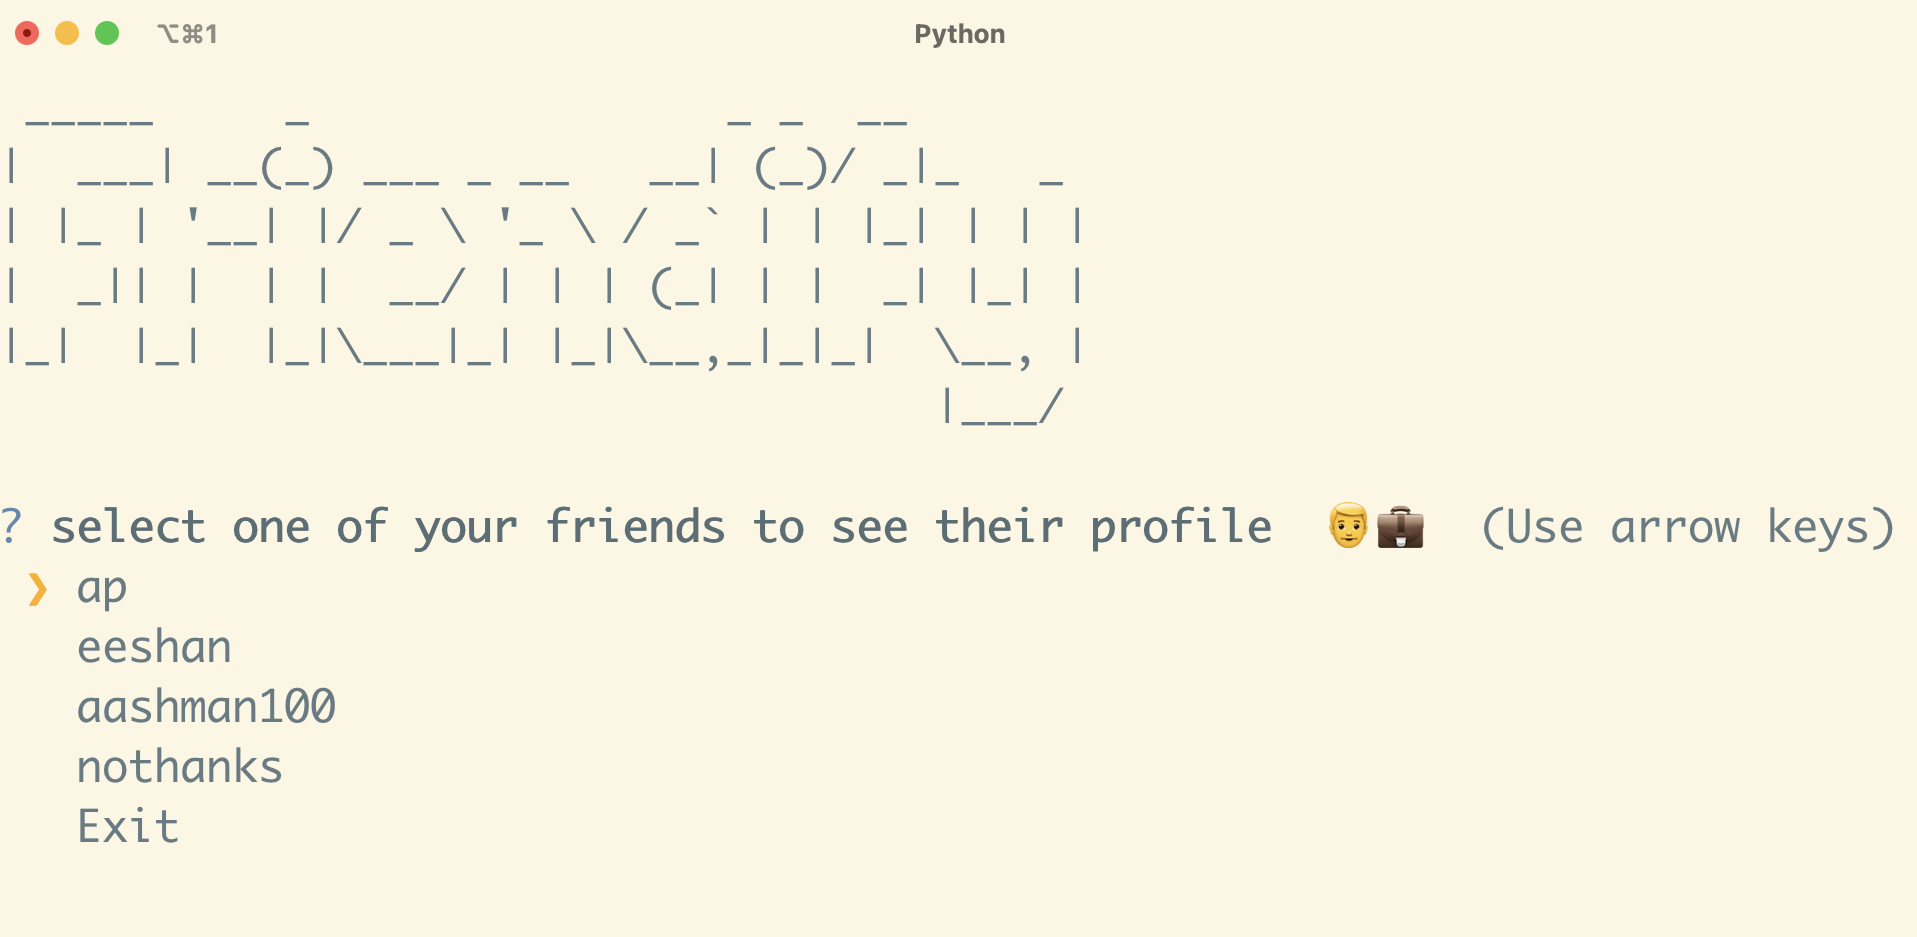
\includegraphics[scale = .35]{Images/myfriends.png}
       \end{center}
       
       From here you can navigate to any of the friends and view their profile. This is how it should look: 
       
             \begin{center}
             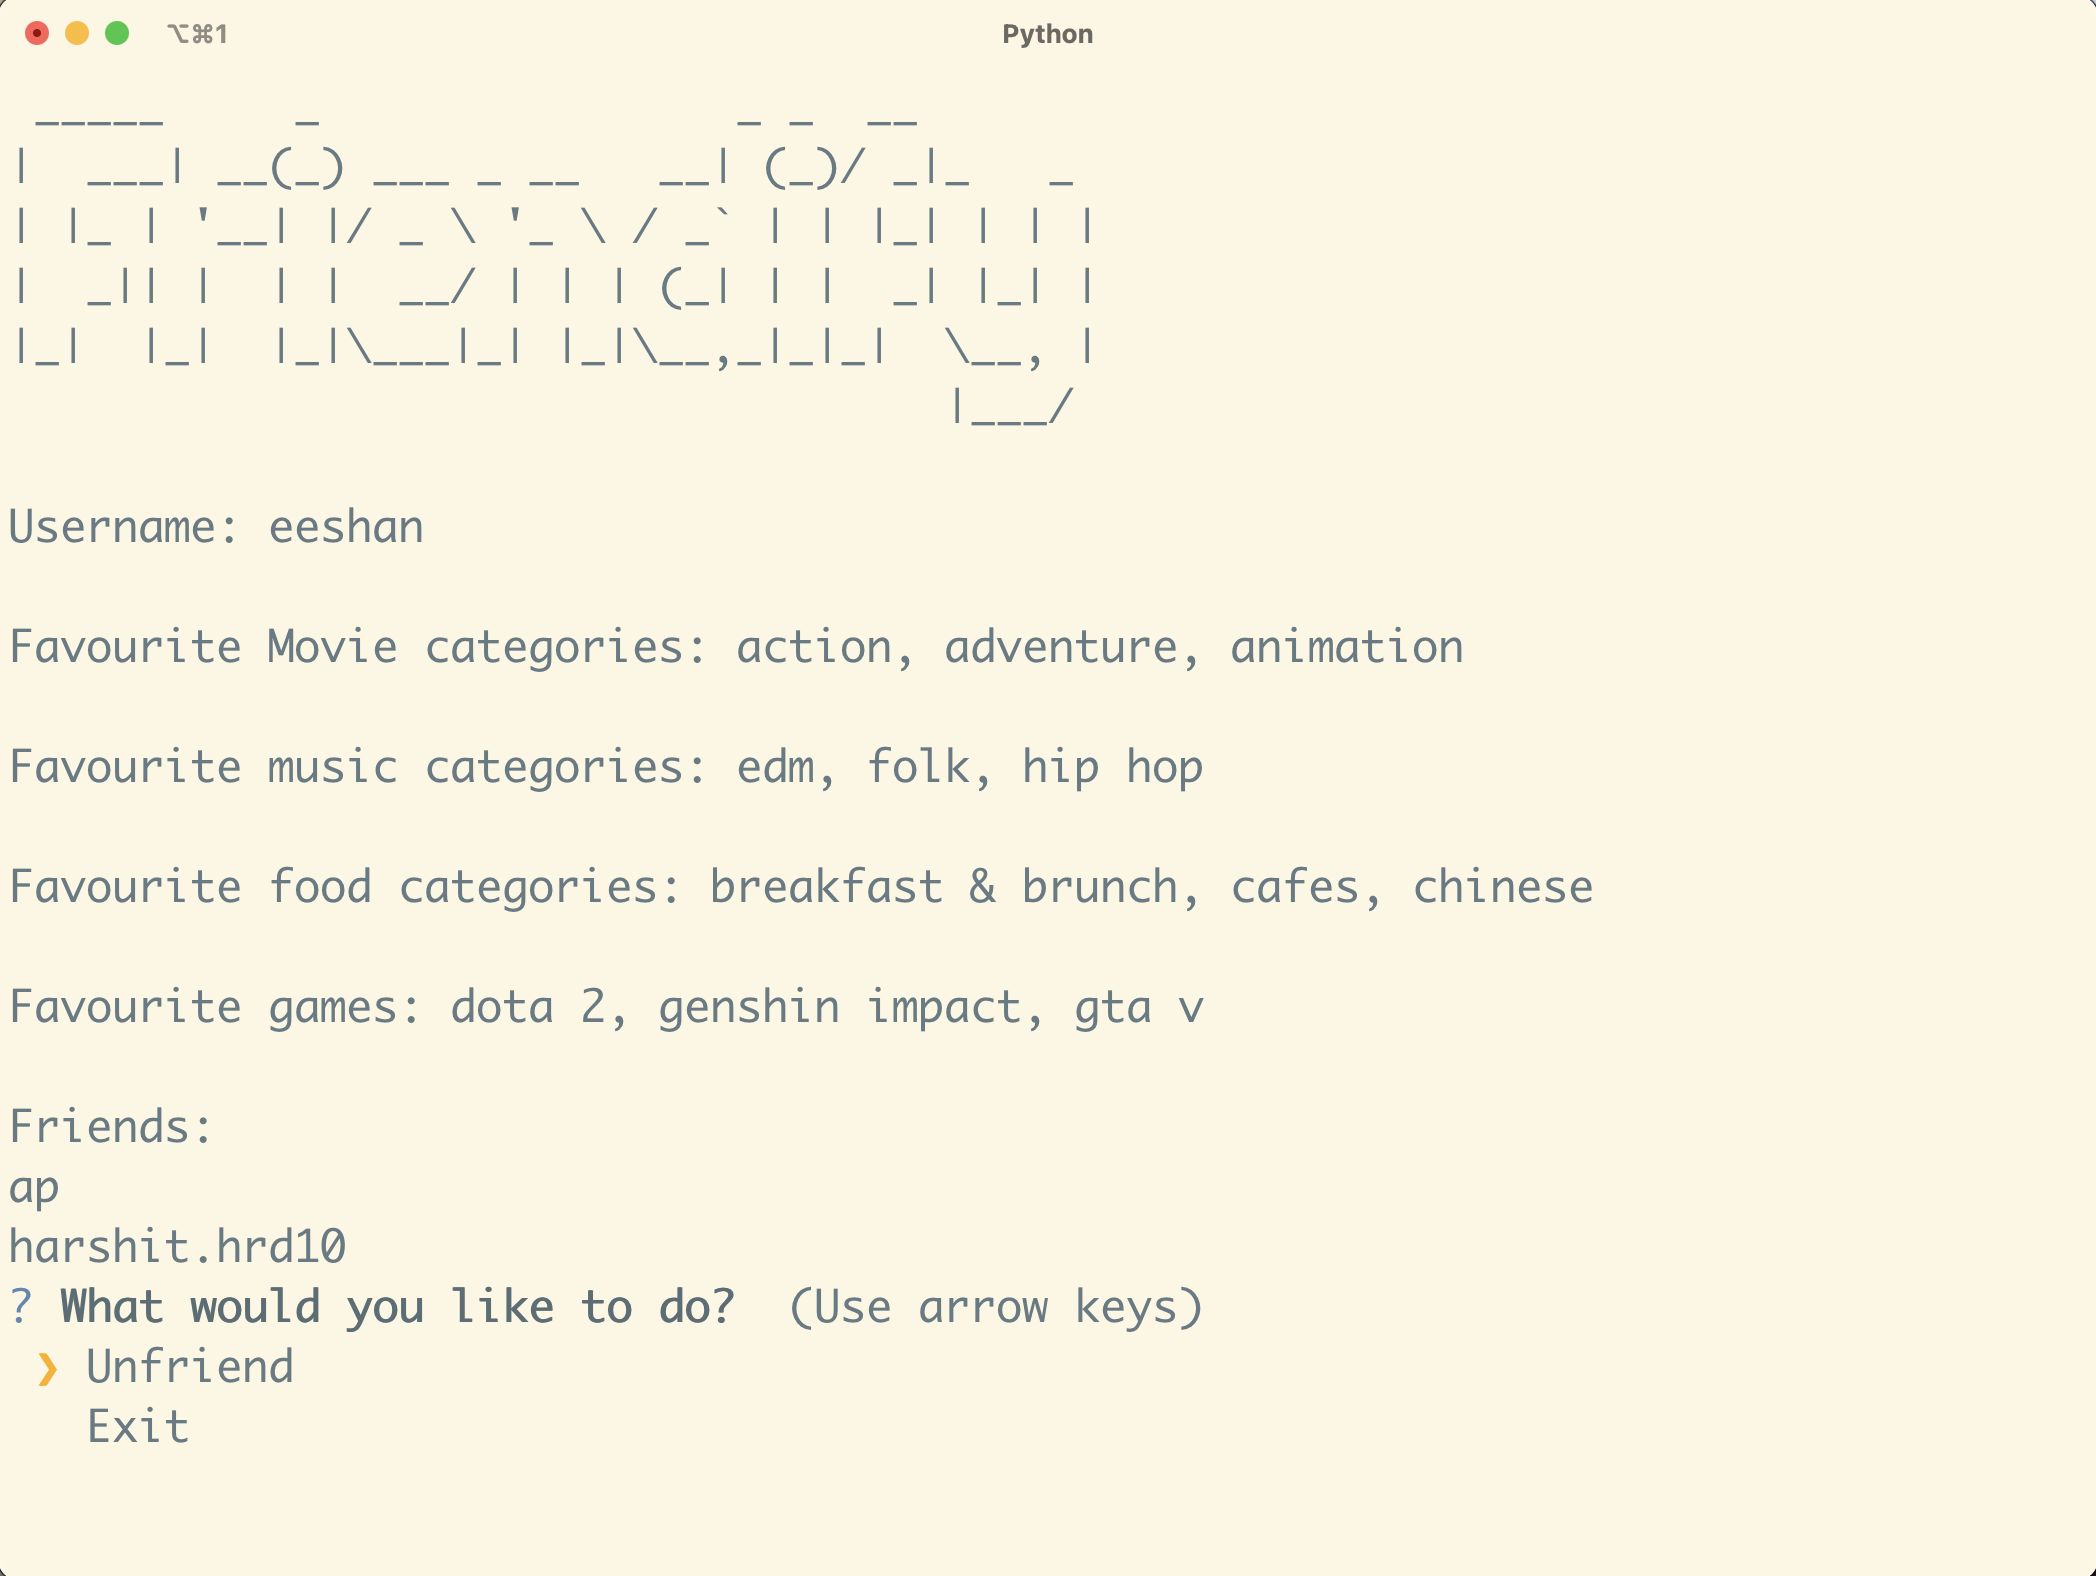
\includegraphics[scale = .35]{Images/friend-prof.png}
      \end{center}
      
      From here you would have the option to unfriend the user, or exit. If you choose to unfriend the user, the user would be removed from your friend list and you would be navigated back to your friends list. \newpage 
      
      \item {\bf Search for people} : This feature allows you to search for people using the app. As you select the feature you would be navigated to a screen which looks like: 
      
      \begin{center}
             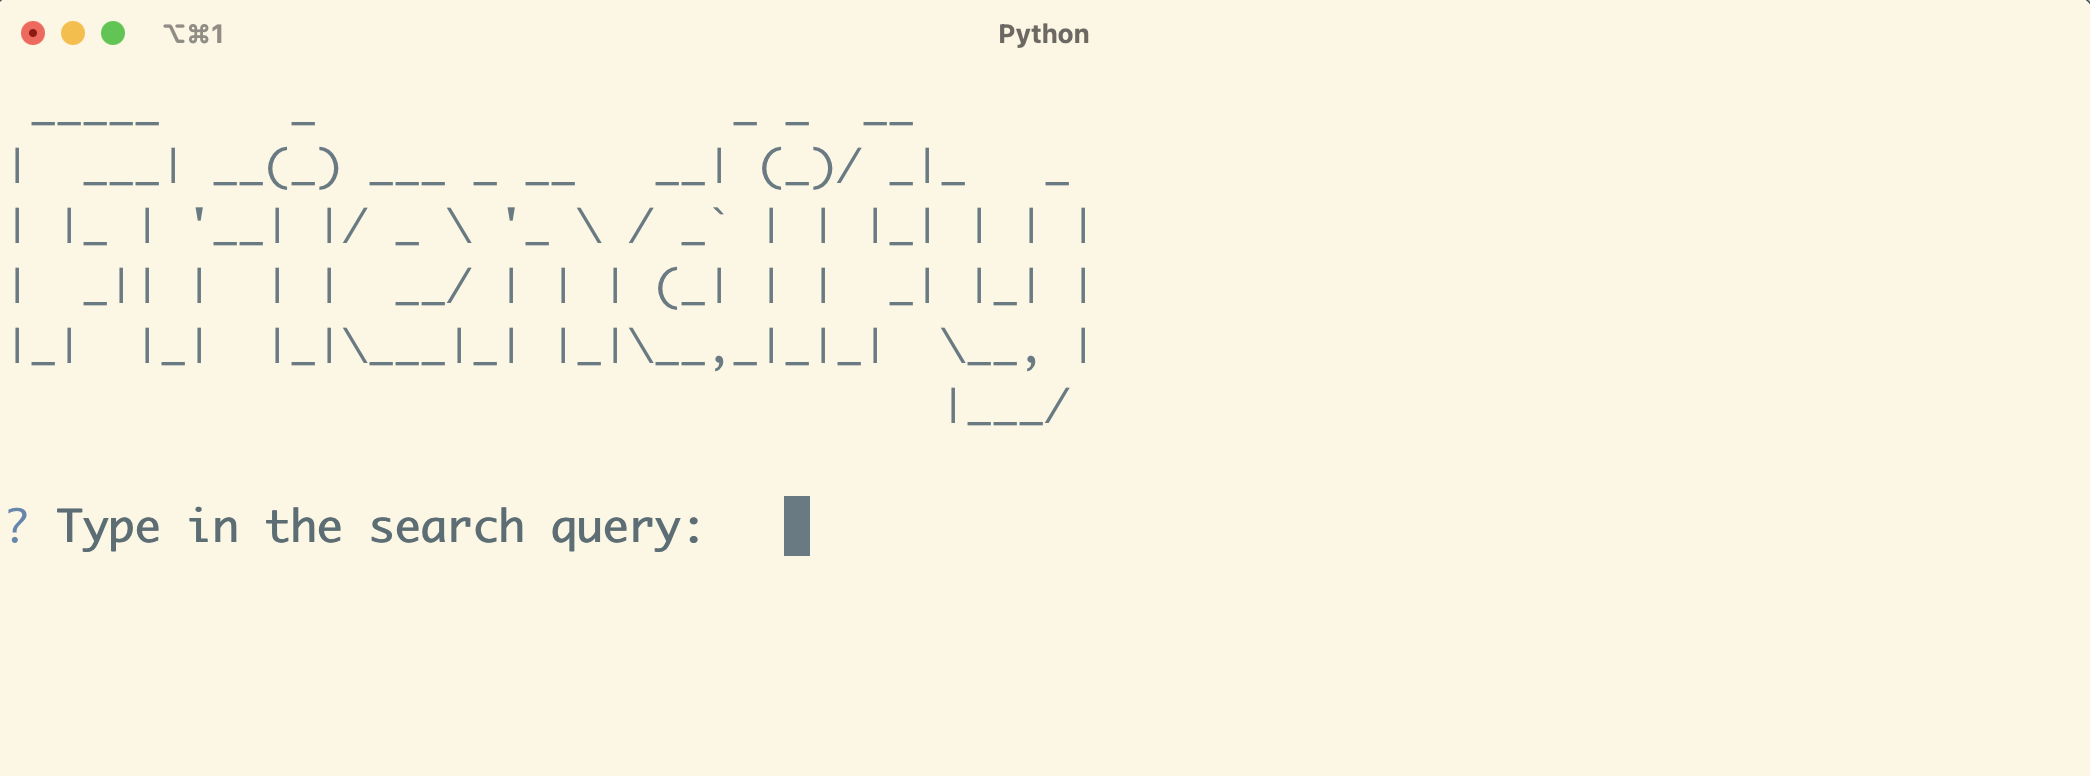
\includegraphics[scale = .35]{Images/query-search.png}
      \end{center}
      
      You have to type the username of the user you are trying to search for, and you will get the top 10 results matching that query. This is how it looks:
      
       \begin{center}
             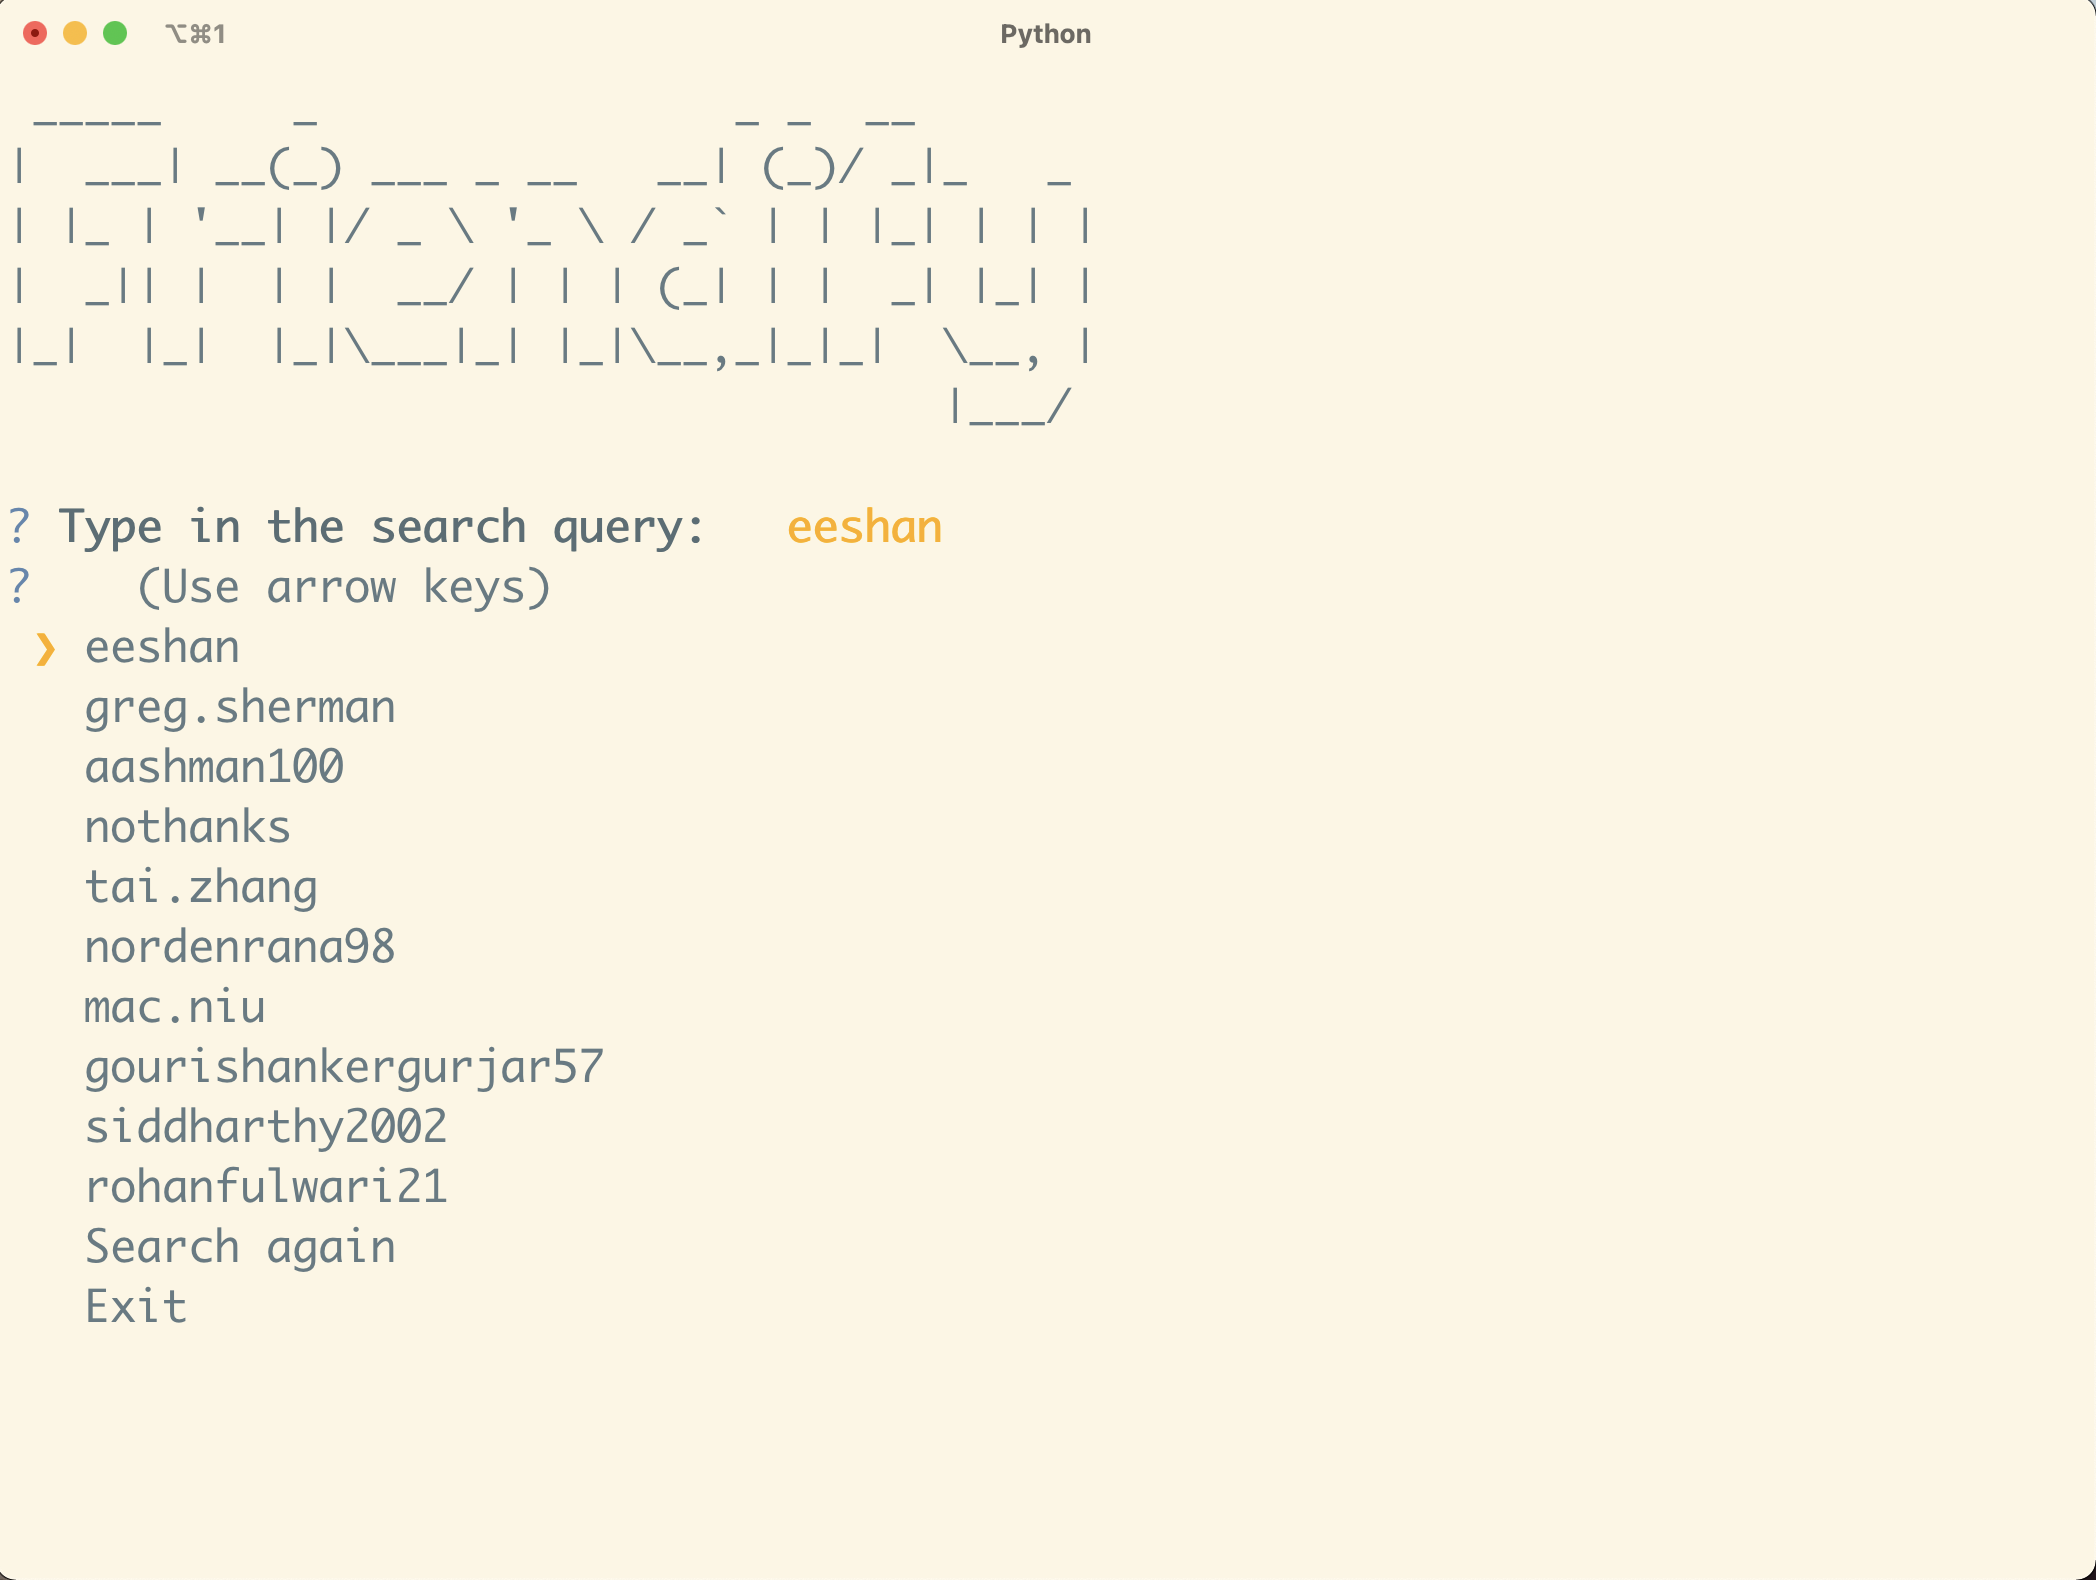
\includegraphics[scale = .35]{Images/search-results.png}
      \end{center}
      
      Form here you can navigate to any of the users. The screen to which you would navigate would contain the profile of the user and the option to friend and unfriend the user depending on whether they are your friend or not. \\
      
      You also have the option to search again or exit the screen and go back to the home screen. \newpage 
      
      \item {\bf your profile} : this feature shows your profile as seen by other users. this is how it looks:
      
      \begin{center}
             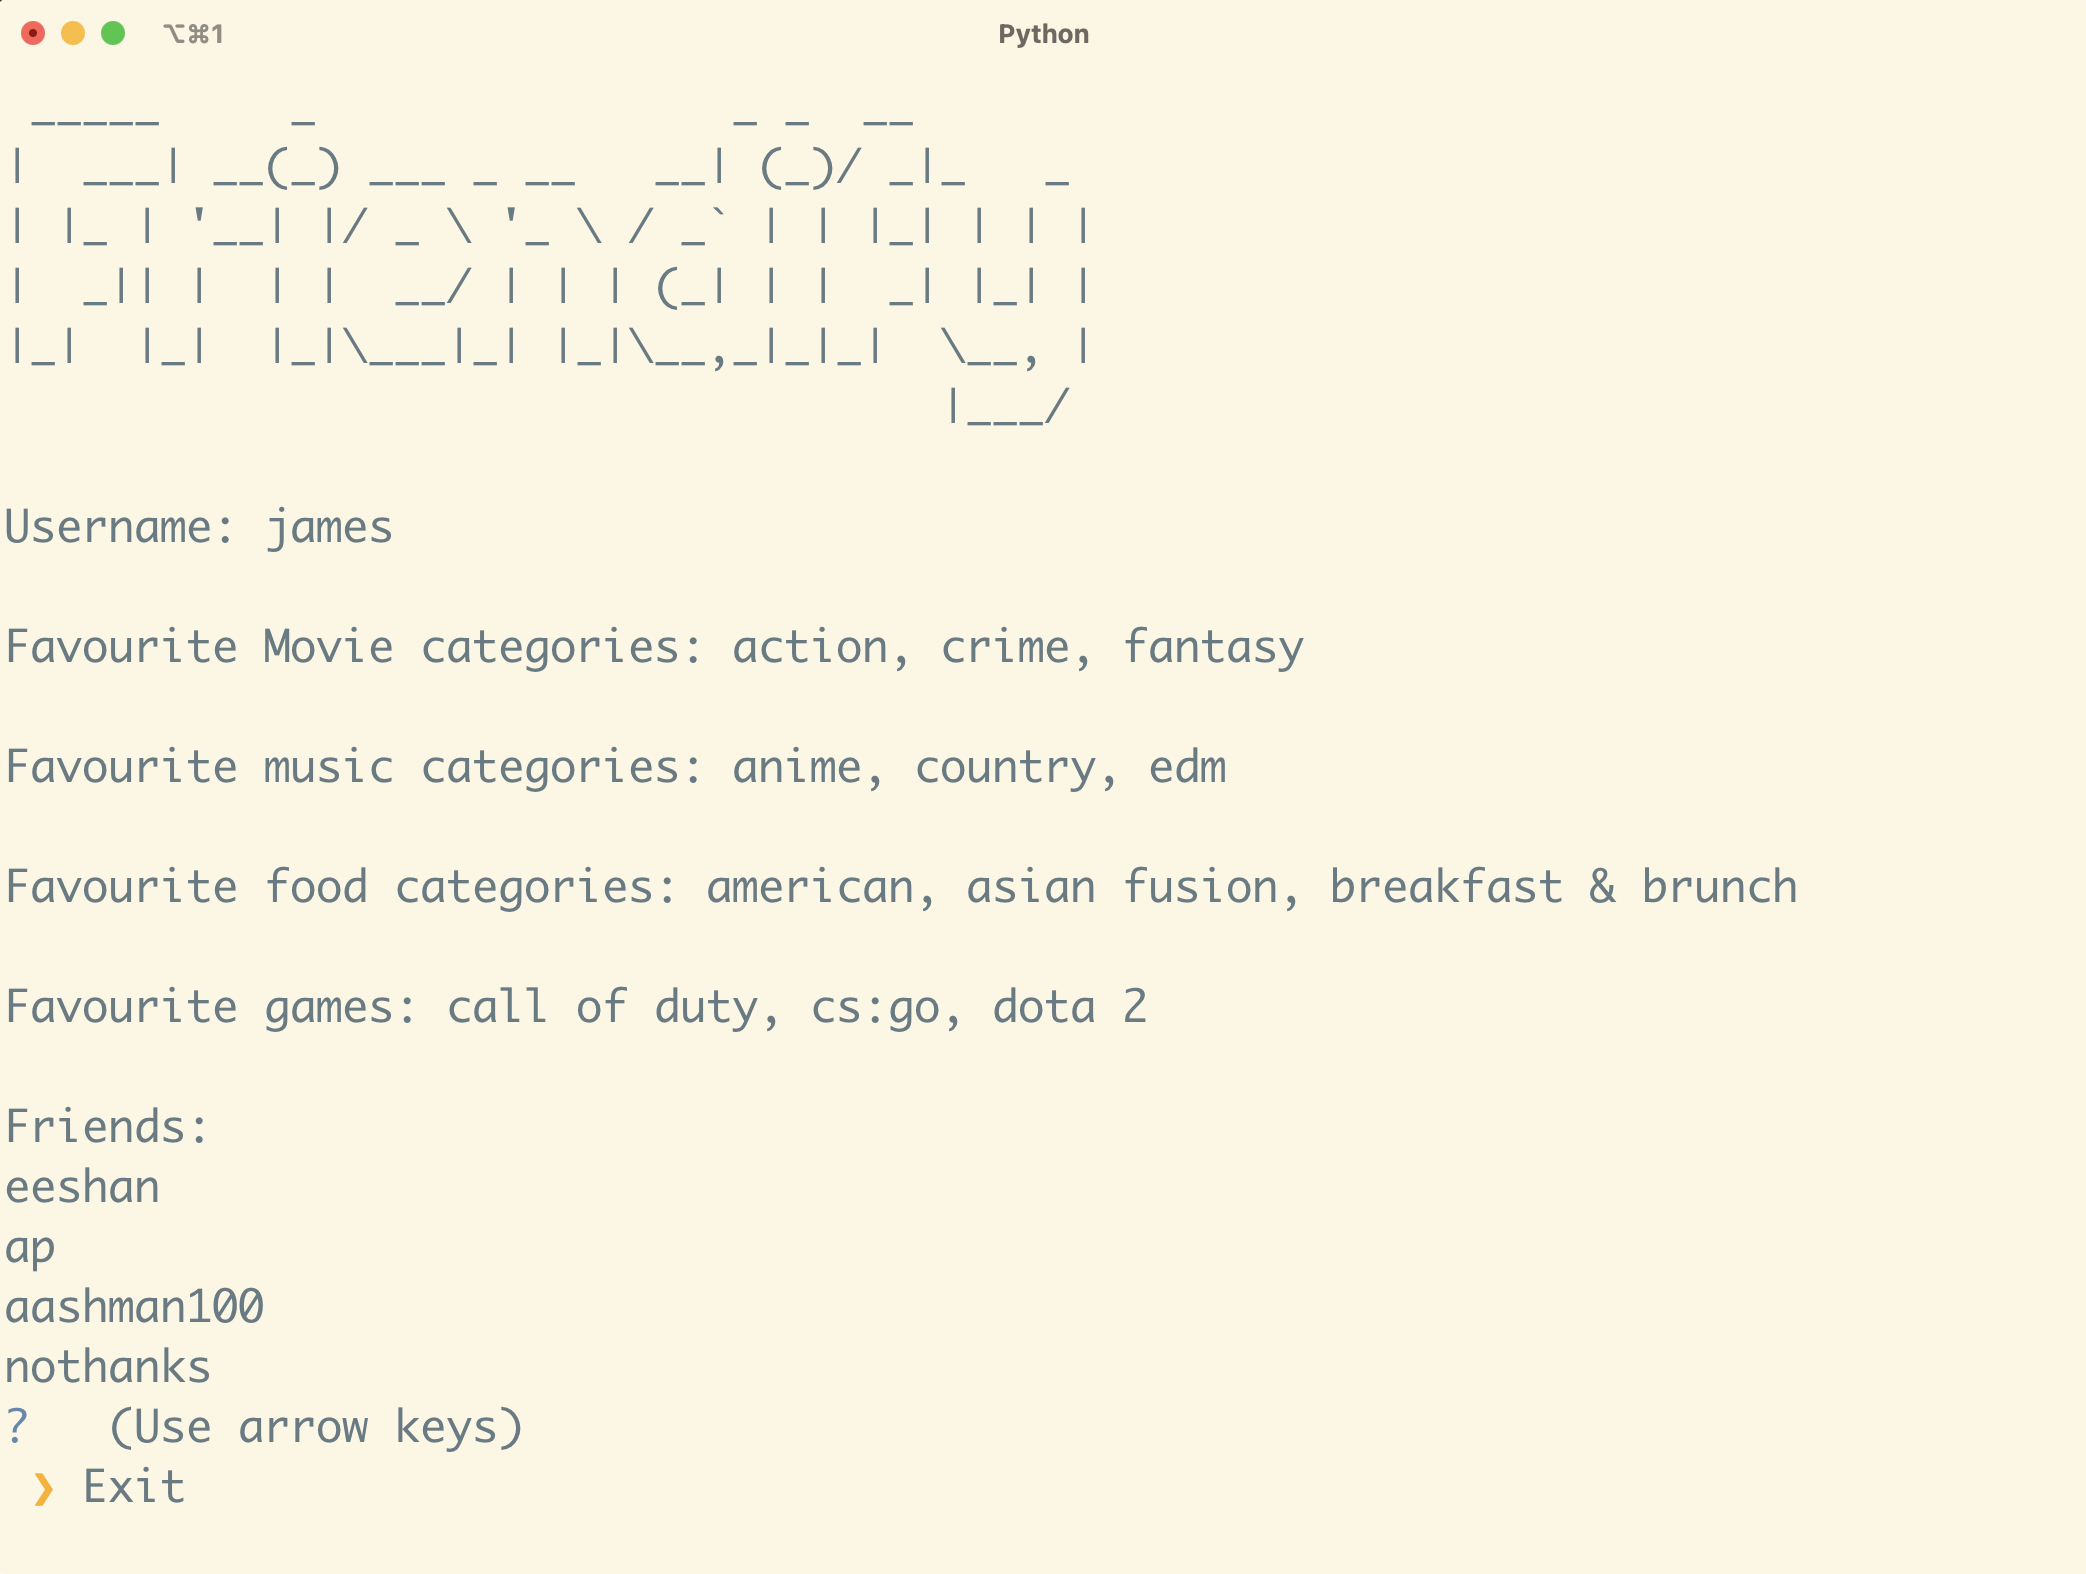
\includegraphics[scale = .3]{Images/profile.png}
      \end{center}
      
      \item {\bf delete account} : Finally you can delete your account by choosing this option. This is how your screen should look:
      
       \begin{center}
             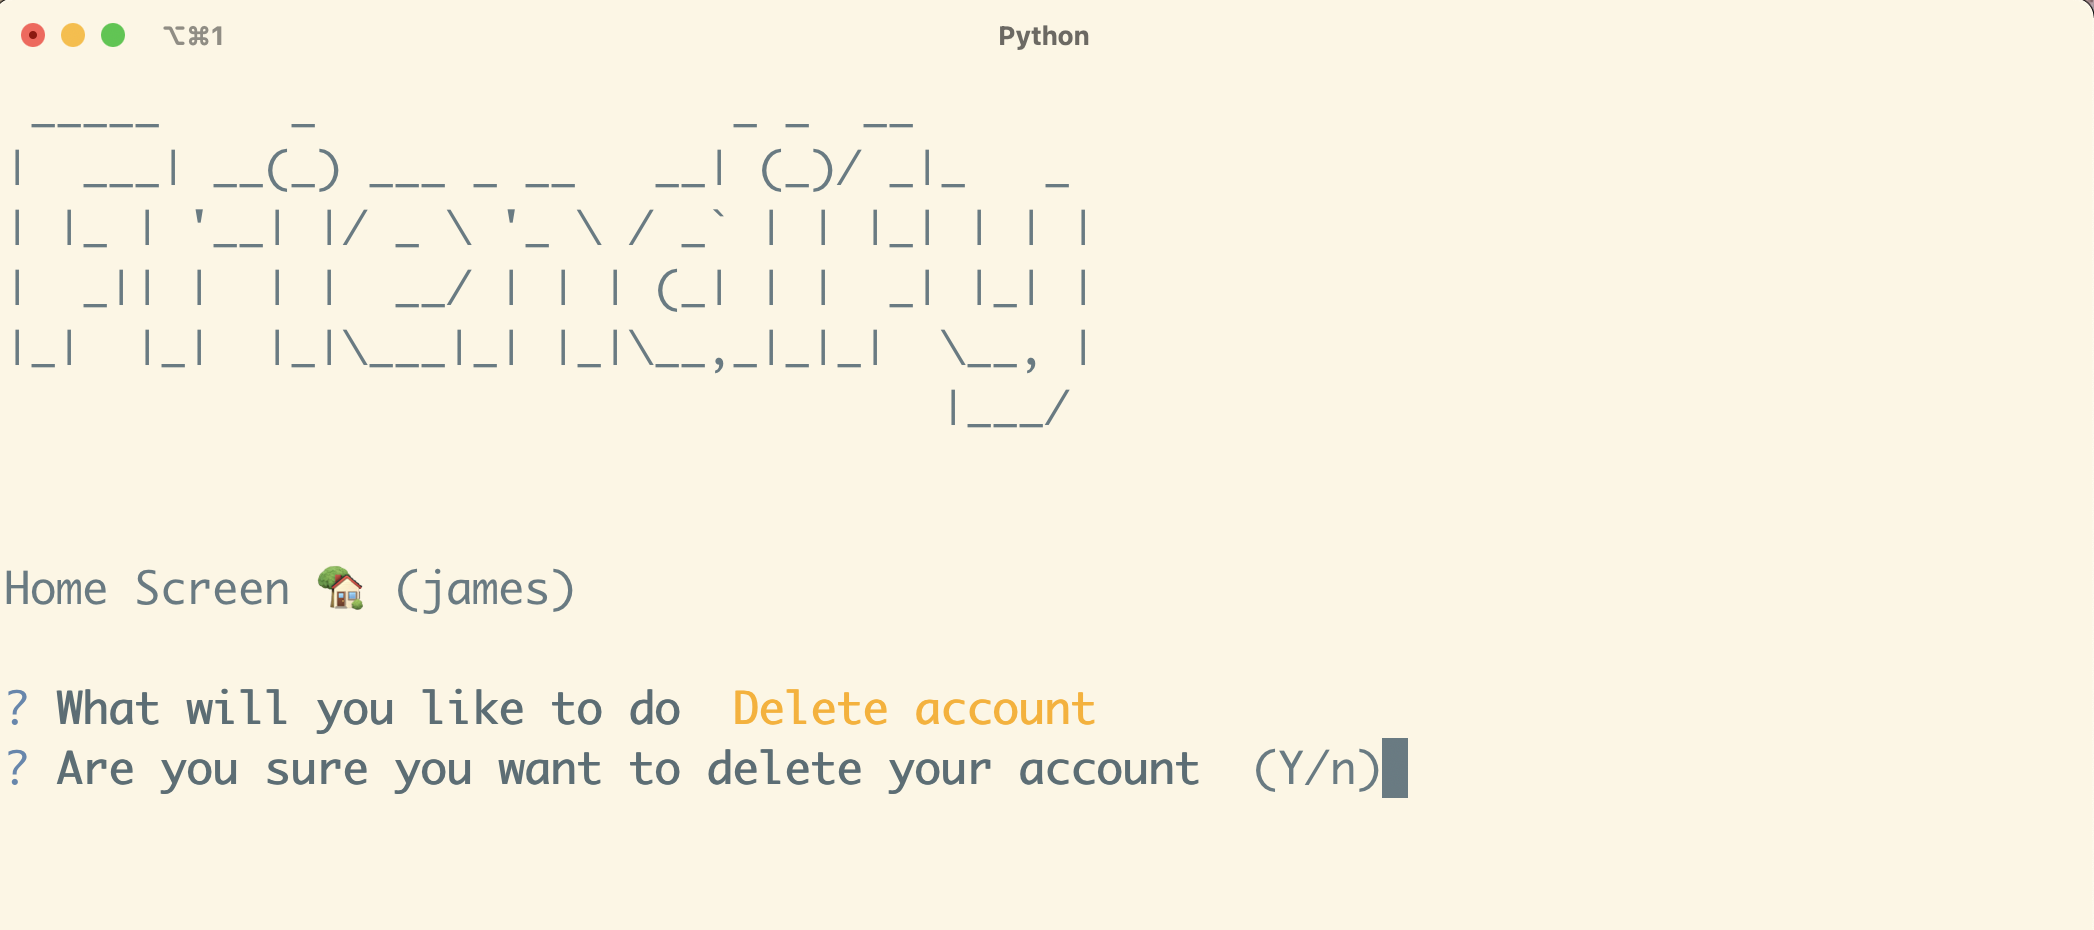
\includegraphics[scale = .32]{Images/delete-confirm.png}
      \end{center}
      
       \begin{center}
             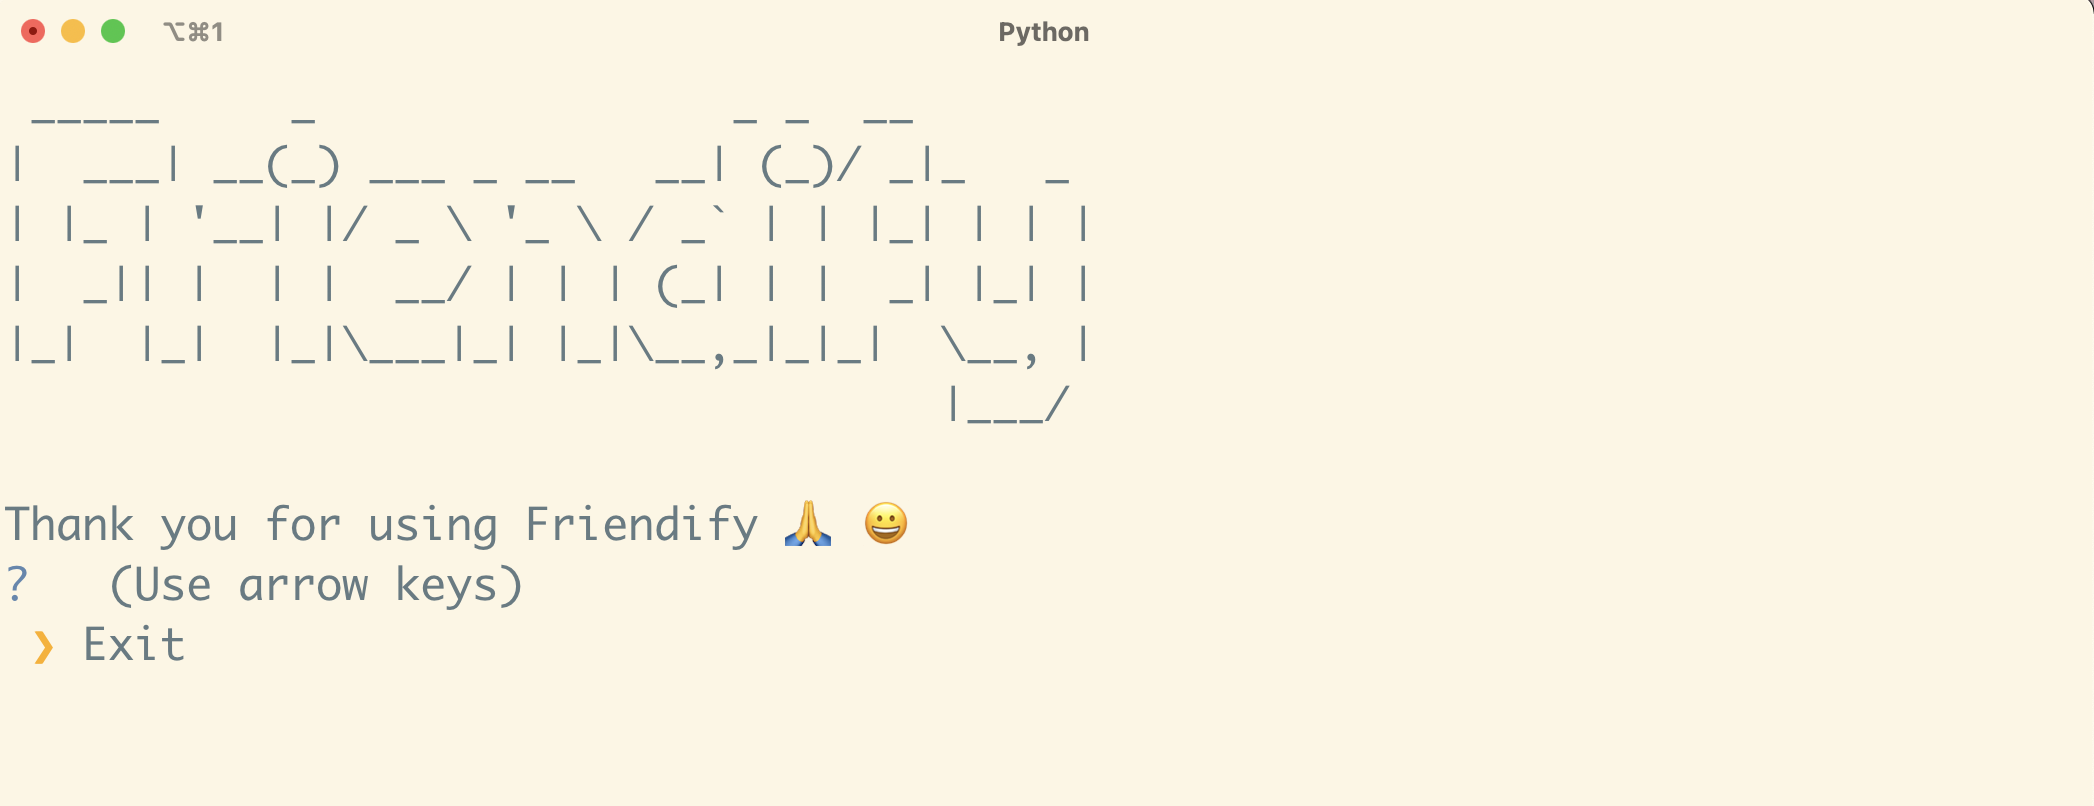
\includegraphics[scale = .32]{Images/delete-tankyou.png}
      \end{center}
      
      From here you would be navigated to the sign-in/register screen.
     
      \end{enumerate}
    
\end{enumerate}



\chapter{Changes from Phase 1 Proposal}

\begin{itemize}
    \item The biggest change we added is the method of recommending friends. Previously our plan was to build up a recommendation tree which looked something like this:
    
    \begin{center}
             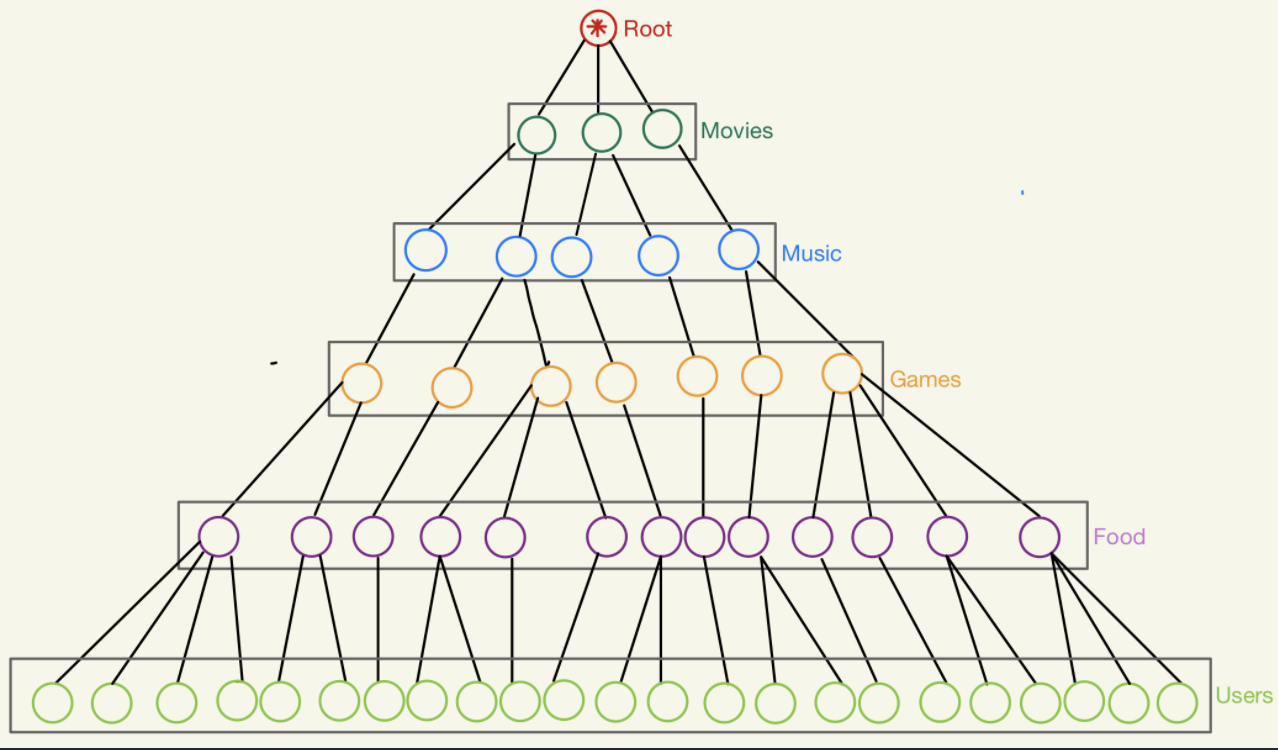
\includegraphics[scale = .5]{Images/tree.png} 
      \end{center}
    
    We concluded that this approach was not very useful in our case.\\
    
    This is because the order of the preferences mattered. \\
    
    For instance, using the tree method (as suggested in Phase 1), a user would get different recommendations based on whether his preferences of movies were placed above or below his preferences of games in the recommendation tree. \\
    
    This led to some of the preferences, not being searched in the tree, which  in-turn led to poor recommendations and poor matching scores. \\
    
    Instead, by using graphs to recommend friends, every possible preference was taken into account while recommending friends. This is how it looks now:
    
    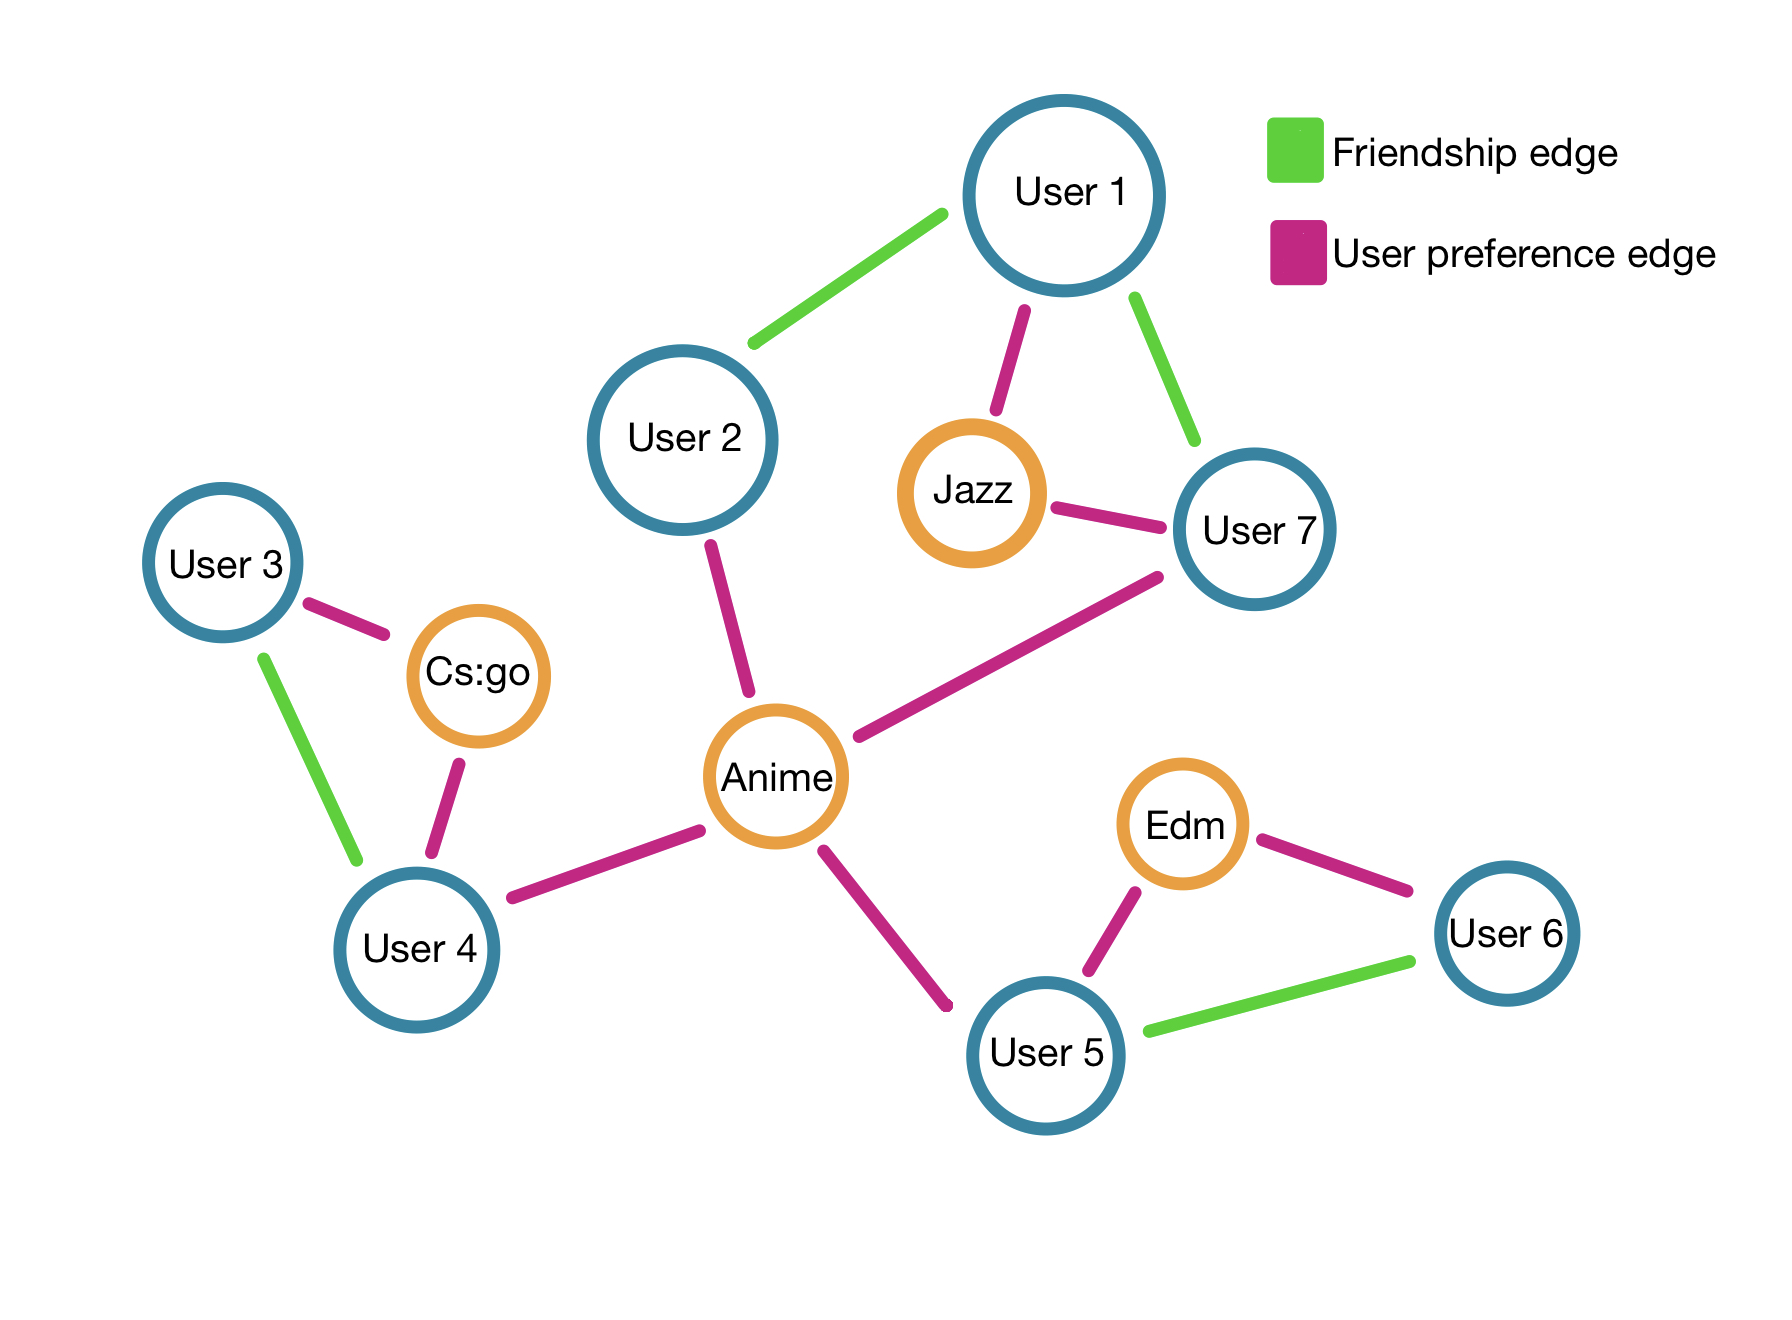
\includegraphics[scale = .2]{Images/graph.jpeg}
    
    \item We also added the feature to search for people using the app - which was not previously present in our proposal \\
    
    \item Further, we added the feature of displaying the similarity score while showing/visualizing our friend recommendations.\\
    
    \item We also added the feature of visualizing our friend network in different architectures (of graph) - like cose, circle, bredthfirst etc.\\
    
    \item Additionally, we added the feature to handle different friends and their user accounts.
\end{itemize}

\chapter{Discussion}

% Yes - You can see friend recommendations (percentage)
%     you can see graph
%     you can see preferances 
%     you can see friends of friends
%     you can connect


The main problem which people face during this pandemic is connecting with people and making friends.\\
We believe that the results and working of this app does help address the problem which we introduced at the beginning of our proposal.\\
Our app helps people connect with each other based on their interests and preferences. \\
Using our app, people can see their friend recommendations, visualize their friend network as a graph, add/remove friends, change their personal preferences (movies, food, games etc.) and do a lot more.\\
Such healthy online interaction is vital for the mental health and well-being of an individual in this time of social isolation.\\
In view of the above points, we feel that our app helps address this issue in a meaningful way.\\
    
    
{\bf Some limitations/problems we encountered -}

\begin{itemize}
    \item Initially, we could not find any dataset online, hence we had to conduct a survey. The response to our survey was also not great, since approximately 50 people responded.
    
    \item To make the online app, we had to use firebase. We encountered several HTTP errors in order to make this an online application. Also, we were not able to use authentication via passwords. since firebase\_admin (official firebase python lib) did not have those options for python (or we were not able to find it).
    
    \item At the beginning, we were using trees to recommend friends.  This led to some of the user preferences, not being searched in the tree, which  in-turn led to poor recommendations and poor matching scores.
    Later, by using graphs to recommend friends, we were able to account for every possible user preference while recommending friends
    % but we were not getting good recommendations although we should be getting them. The matching scores were as high as 7 to 8 percent. We then figured out that his was occurring due to the reason that trees are special type of graphs and do not have any cycles. We then used graphs to solve the problem and now we get as high as 50-55 percent match scores.
    
    \item While using the dash app for visualization, the visualization would not open automatically. Thus, we had to find a way open it using the web-browser library. We are still not able to shut the site down automatically, because the web-browser library can not do that. We can instead kill the localhost site using some terminal commands.
    
    % \item While searching for people, our app only takes into account the similarity score and the user ids to give the top search results. We tried to construct a model which takes into account not only the similarity between different user preferences, but also the similarity score between the user who is conducting the search and the search results. However, we were not able to construct a balance between the two factors.
    
    \item Currently, our app is a terminal app and the UI runs on the terminal. We tried  to run it on the the console, but since Pyinquiere and Cutie make use of the terminal, this process was difficult for us to implement and thus we were unable to do this.
\end{itemize}



{\bf Future exploration -}

\begin{itemize}
     \item We plan on adding authentication via password to all user accounts to increase security.
     \item We also plan on introducing a feature which would allow users to make their accounts public or private, based on their choice. This feature would help users maintain their privacy.
     \item We plan on adding a `friend request' feature, instead of directly allowing the users to add other people without their permission.
     \item We also plan to add a built-in chat system in the future.
\end{itemize}




\chapter{References}

Libraries:

\begin{itemize}
    \item  \href{https://firebase.google.com/docs/reference/admin/python/firebase_admin}{\color{blue} Firebase admin} 
    \item  \href{https://github.com/eeshannarula29/Friendify}{\color{blue} PyInquirer}
    \item  \href{https://pypi.org/project/cutie/}{\color{blue} Cutie}
    \item  \href{https://www.geeksforgeeks.org/python-ascii-art-using-pyfiglet-module/}{\color{blue} Pyfiglet}
    \item  \href {https://plotly.com/python/network-graphs/}{\color{blue} Dash and Plotly}
\end{itemize}

Sources:

\begin{itemize}
    \item Source 1 - https://www.healthline.com/health-news/people-with-covid-19-more-likely-to-develop-depression-anxiety-and-dementia\#How-the-new-coronavirus-affects-the-mind
    
    \item Source 2 - https://www.ncbi.nlm.nih.gov/pmc/articles/PMC7306546/\#:\\~:text=Quarantine\%20and\%20social\%20distancing\%20are,and\%20mental\%2Dhealth\%20related\%20repercussions
    
    \item Source 3 - https://www.kff.org/coronavirus-covid-19/issue-brief/the-implications-of-covid-19-for-mental-health-and-substance-use/
    
    \item Source 4 - https://oaksatdenville.org/blog/benefits-social-interactions/
\end{itemize}

\newpage


%%%%%%%%%%%%%%%%%%%%%%%%%%%%%%%%%%%%%%%%%%%%%%%%%%%%%%%%%%%%%%%%%%%%%%%%%%%%%%%%%%%%%%%
% Appendix
%%%%%%%%%%%%%%%%%%%%%%%%%%%%%%%%%%%%%%%%%%%%%%%%%%%%%%%%%%%%%%%%%%%%%%%%%%%%%%%%%%%%%%%
% \include{Appendix/appendix} <------ Appendix

\end{document}
